\documentclass[aspectratio=169]{beamer}

\usepackage[T1, T2A]{fontenc}
\usepackage[english, serbianc]{babel}
\usepackage{tikz}
\usepackage[dvipsnames]{xcolor} % for more colors

\usepackage{caption}
\usepackage{subcaption}
\captionsetup[figure]{font=footnotesize, justification=centering}
\captionsetup[table]{font=footnotesize, justification=centering}
\usepackage{booktabs} % for bold lines in table

%\usetikzlibrary{external} % for figure externalization
%\tikzexternalize[prefix=slike/prezentacija/] % activate externalization!

% Color variables
\def \CtrlColor        {darkgray}
\def \BBctrlColor      {RoyalBlue}
\def \PIDctrlColor     {OliveGreen}
\def \DCOColor         {BrickRed}
\def \CtrlDecColor     {brown}
\def \CtrlPreprocColor {RoyalPurple}
\def \ClkDivColor      {Goldenrod}
\def \RstnColor        {BurntOrange}

\definecolor{UniRed}{HTML}{d40019}
\definecolor{UniGreen}{HTML}{3c671d}
\definecolor{UniBlue}{HTML}{0062aa}
\definecolor{UniPurple}{HTML}{69227f}
\definecolor{UniAmber}{HTML}{fcb900}
\definecolor{UniBlack}{HTML}{1b1918}
\definecolor{FinCyan}{HTML}{6fdaf8}
\definecolor{FinGray}{HTML}{c4c5c7}
\definecolor{FinBlack}{HTML}{201d1e}
\definecolor{TocSubsection}{HTML}{1F4D80}

\usetheme{Warsaw}
\usecolortheme{structure}
\setbeamercolor{structure}{fg=UniBlue}
\setbeamercolor{subsection in toc}{fg=TocSubsection}
% \setbeamertemplate{description item}{\makebox[3em][l]{\insertdescriptionitem}}
\setbeamertemplate{headline}{}
\setbeamertemplate{navigation symbols}{}
\setbeamertemplate{section in toc}[square]

\newcommand\numbered{\setbeamertemplate{footline}{\vspace{-12pt}\hfill\usebeamercolor[fg]{page number in head/foot}\usebeamerfont{page number in head/foot}\insertframenumber\,/\,\inserttotalframenumber\kern2pt\vskip2pt}}
\newcommand\samenumbered{\setbeamertemplate{footline}{\vspace{-12pt}\hfill\usebeamercolor[fg]{page number in head/foot}\usebeamerfont{page number in head/foot}\insertframenumber\,/\,\inserttotalframenumber\kern2pt\vskip2pt}\addtocounter{framenumber}{-1}}
\newcommand\unnumbered{\setbeamertemplate{footline}{}\addtocounter{framenumber}{-1}}

% Избор логотипа на насловној страни:
% \titlelogouni --- универзитетски лого
% \titlelogofin --- факултетски лого
% \titlelogoboth --- оба логотипа
\newcommand{\titlelogofin}{\def\titlelogo{\begin{figure}
\includegraphics[height=55pt]{./slike/grb/finkg_logo}\end{figure}}}
\newcommand{\titlelogouni}{\def\titlelogo{\begin{figure}
\includegraphics[height=55pt]{./slike/grb/unikg_logo}\end{figure}}}
\newcommand{\titlelogoboth}{\def\titlelogo{\begin{figure}
\includegraphics[height=55pt]{./slike/grb/unikg_logo}\qquad
\includegraphics[height=55pt]{./slike/grb/finkg_logo}\end{figure}}}

\makeatletter
\newcommand*{\engl}[2][\@empty]{%
    \edef\theacronym{#1}%
    (енгл. \foreignlanguage{english}{\emph{#2}%
    \ifx\theacronym\@empty \else , #1\fi})%
}
\makeatother

\titlelogoboth

% Избор логотипа на подножју слајдова:
% \footlogouni --- универзитетски лого
% \footlogofin --- факултетски лого
% \footlogo{...} --- произвољна слика
\newcommand{\footlogo}[1]{\setbeamertemplate{background canvas}{%
\ifnum\insertframenumber>0
    \begin{tikzpicture}[overlay, remember picture]
        \node[anchor=south west] at (current page.south west) {\includegraphics[width=20pt]{#1}};
    \end{tikzpicture}%
\fi}}
\newcommand{\footlogouni}{\footlogo{slike/grb/unikg_logo.pdf}}
\newcommand{\footlogofin}{\footlogo{slike/grb/finkg_logo.pdf}}

\footlogouni


\title{\Large{Пројектовање синтетизабилне сведигиталне фреквенцијски\\затворене петље са широким опсегом подешавања\\до учестаности од 640\texorpdfstring{\,}{ }MHz}}

\author{Ђорђе Гачић\texorpdfstring{\vspace{-1em}}{}}%
\institute{\textbf{Катедра за електротехнику и рачунарство}\\Факултет инжењерских наука Универзитета у Крагујевцу%
\vspace{7pt}\titlelogo\vspace{-9pt}}
\date{Крагујевац, \today}

% Приказивање садржаја између поглавља
% \AtBeginSection[]{%
%     \begin{frame}{\contentsname}
%         \tableofcontents[currentsection, hideallsubsections]
%     \end{frame}%
% }

% Abbreviation variables
\def \PLL  {PLL} % phase-locked loop
\def \FLL  {FLL} % frequency-locked loop
\def \DLL  {DLL} % delay-locked loop
\def \DCO  {DCO} % digitally controlled oscillator 
\def \PID  {ПИД} % proportional-integral-derivative
\def \P    {П}   % proportional
\def \I    {И}   % integral
\def \D    {Д}   % derivative
\def \FCW  {FCW} % frequency control word
\def \PVT  {PVT} % process-voltage-temperature
\def \HLLS {HLLS} % high-low level shifter
\def \LHLS {LHLS} % low-high level shifter

\begin{document}
\numbered

{\unnumbered
\begin{frame}
   \titlepage
\end{frame}}

\section*{Садржај}
\begin{frame}{\secname}
    \scriptsize
    \tableofcontents[hideallsubsections]
\end{frame}

\section{Увод и мотивација}
\begin{frame}{\secname}
    \begin{itemize}
        \item Постоји велики број чипова који захтијевају генератор такта, за чију имплементацију се обично користи фазно затворена петља (\PLL).
        \item Међутим, да ли је \PLL\ увијек неопходан?
	\item Можда је довољна фреквенцијски затворена петља (\FLL)?
	%\item Испоставља се да није, и да је сасвим довољна фреквенцијски затворена петља (FLL) која само множи улазну учестаност, без да води рачуна о фази такта.
    \end{itemize}
    
    \bigskip
    \centering
    \hspace{-1cm}
    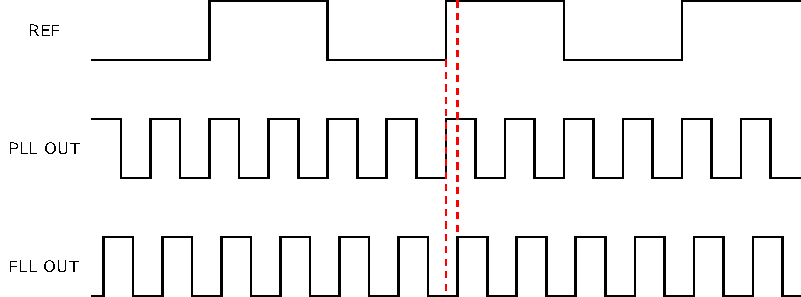
\includegraphics[scale=0.8]{slike/prezentacija/fll_pll_fref_fout.pdf}
\end{frame}

\begin{frame}{\secname}
    \begin{center}
	    \color{BrickRed}Дигитални \color{black} или \color{RoyalBlue} аналогни \color{black} FLL
    \end{center}	  
  	 \medskip    
    \begin{columns}[t]
        \begin{column}{0.5\textwidth}
			\color{black} Предности дигиталног \FLL-a:
			\begin{itemize}
			    \color{BrickRed}
				\item мања површина
				\item отпорност на \PVT\ промјене
				\item прилагодљивост различитим технологијама
				\item већа скалабилност и могућност параметризације
				\item једноставније и брже пројектовање
			\end{itemize}
		\end{column}
		\bigskip
		\begin{column}{0.5\textwidth}
			\color{black} Предности аналогног \FLL-a:
			\begin{itemize}
				\color{RoyalBlue}
				\item већа максимална учестаност
				\item боља резолуција учестаности
			\end{itemize}
		\end{column}
	\end{columns}
	\bigskip
	\begin{center}
		Кад год захтјеви то дозвољавају, пожељно је користити дигитални \FLL!
    \end{center}	
\end{frame}

\section{Дигитална фреквенцијски затворена петља (\FLL)}
\begin{frame}{\secname}
    \small
    \centering
    \hspace{-0.8cm}
    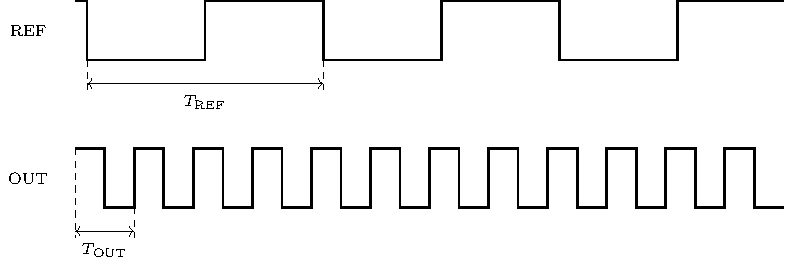
\includegraphics[scale=0.8]{slike/prezentacija/fll_fref_fout.pdf}
    \vspace{-0.2cm}
    \begin{equation}
        f_\text{REF} = \frac{1}{T_\text{REF}}
    \end{equation}
    \begin{equation}
        f_\text{OUT} = \frac{1}{T_\text{OUT}}
        \vspace{0.3cm}
    \end{equation}
    \begin{equation}
	f_\text{OUT} = \text{FMUL} \cdot f_\text{REF}
    \end{equation}
\end{frame}

\subsection{Структура}
\begin{frame}{Дигитални \FLL: \subsecname}
	\centering
	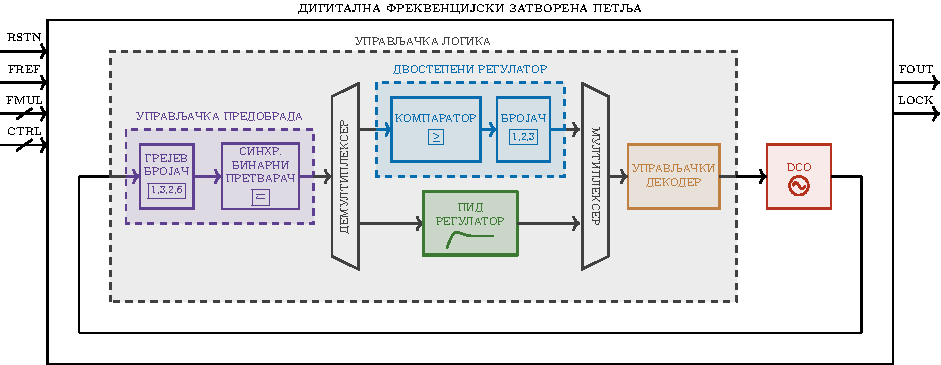
\includegraphics[scale=0.85]{slike/prezentacija/FLL.pdf}
	\medskip
	\begin{itemize}
		\item Управљачка логика
		\item Дигитално контролисани осцилатор (DCO)
	\end{itemize}
\end{frame}

\section{Дигитално контролисани осцилатор (\DCO)}
\begin{frame}{\secname}
    \vspace{-0.6cm}
    \begin{columns}[t]
        \begin{column}{0.25\linewidth}
        	\begin{center}
	            
\includegraphics[scale=2]{slike/prezentacija/DCO_blk.pdf} 
	        \end{center}
        \end{column}
        \begin{column}{0.75\linewidth}
        	\begin{center}
            	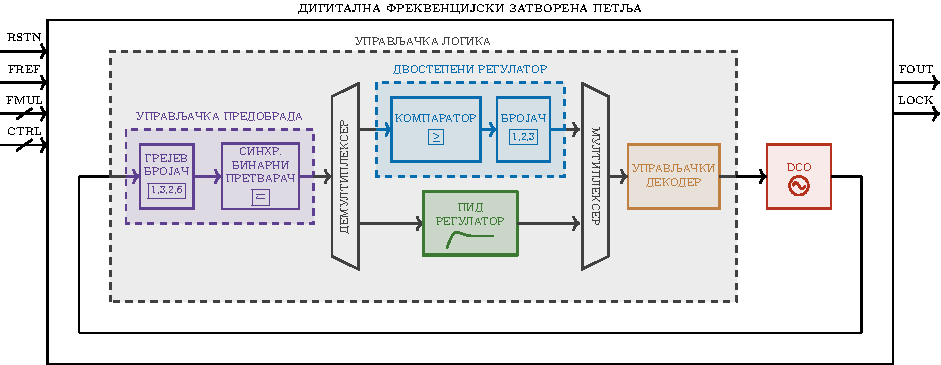
\includegraphics[scale=0.5]{slike/prezentacija/FLL.pdf}
            \end{center}
        \end{column}
    \end{columns}
    \bigskip
    
    \begin{itemize}
	\item У срцу сваке фазно затворене петље налази се осцилатор, који има критичну улогу у постизању жељених перформанси система.
        \medskip
        \item Пројектован је као прстенасти \DCO\ заснован на матрици тростатичких инвертора, са одвојеним напоном напајања.
    \end{itemize}
\end{frame}

\subsection{Инверторски прстен}
\begin{frame}{\DCO: \subsecname}
    \begin{columns}[t]
        \begin{column}{0.5\linewidth}
        	\begin{center}
	            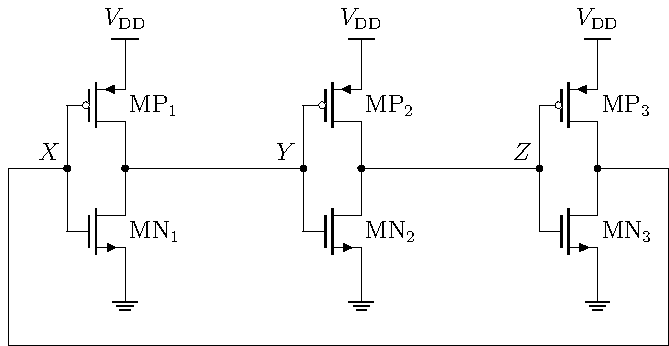
\includegraphics[scale=0.5]{slike/prezentacija/inv_ring_osc_1.pdf} 
	        \end{center}
        \end{column}
        \begin{column}{0.5\linewidth}
        	\begin{center}
            	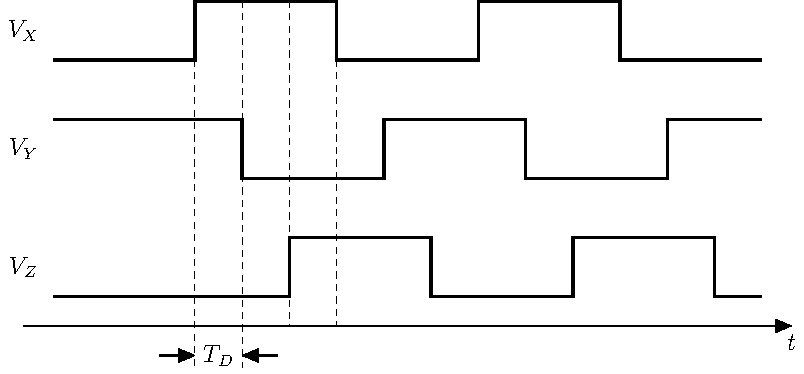
\includegraphics[scale=0.5]{slike/prezentacija/inv_ring_osc_2.pdf}
            \end{center}
        \end{column}
    \end{columns}
    \bigskip
    \vspace{0.5cm}
    \small
    \begin{equation}
        f_\text{OSC} = \frac{1}{6T_D} \nonumber
    \end{equation}
\end{frame}

\subsection{Реалан облик сигнала за тростепени и петостепени прстен}
\begin{frame}{\DCO: \subsecname}
    \begin{columns}[t]
        \begin{column}{0.5\linewidth}
		\begin{itemize}
		    \item тростепени прстен
		\end{itemize}
		\medskip
        	\begin{center}
	            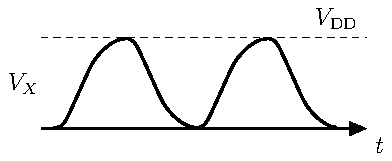
\includegraphics[scale=0.6]{slike/prezentacija/inv_ring_osc_3_1.pdf} 
	        \end{center}
		\begin{equation}
	   	    f_\text{OSC} = \frac{1}{6T_D} \nonumber
		\end{equation}
        \end{column}
        \begin{column}{0.5\linewidth}
		\begin{itemize}
		    \item петостепени прстен
		\end{itemize}
		\medskip
        	\begin{center}
            	    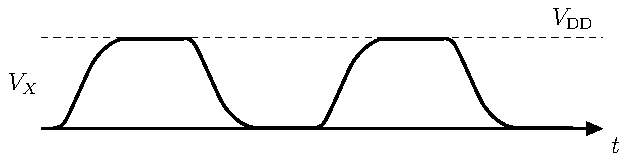
\includegraphics[scale=0.6]{slike/prezentacija/inv_ring_osc_3_2.pdf}
                \end{center}
		\begin{equation}
	   	    f_\text{OSC} = \frac{1}{10T_D} \nonumber
		\end{equation}
        \end{column}
    \end{columns}
    \bigskip
    \vspace{0.5cm}
    \begin{itemize}
	\item Повећањем броја степени (фаза) учестаност осциловања се смањује.
    \end{itemize}
\end{frame}

\subsection{Прстенасти осцилатор}

\def \DCOformula {	
	\begin{itemize}
        \item Формула за учестаност осциловања инверторског прстенастог осцилатора:
            \begin{equation}
                f_\text{osc} = \dfrac{1}{2Nt_\text{d}} \approx \dfrac{I_\text{d}}{2NC_\text{load}V_\text{DDL}}\nonumber
            \end{equation}
            \vspace{-0.25cm}
            \begin{itemize}
                \item $N$ је број тростатичких инвертора у једном прстену (број степени, тј. фаза)
                \item $t_\text{d}$ је кашњење ћелије \DCO-а која садржи тростатички инвертор
                \item $I_\text{d}$ је струја кроз један тростатички инвертор
                \item $C_\text{load}$ је капацитивно оптерећење тростатичког инвертора
                \item $V_\text{DDL}$ је напон напајања \DCO-а
            \end{itemize}
	\end{itemize}  
}
% subframe: As more inverters in each stage are turned on by the FLL control logic, the current driving strength of the stage increases while its capacitive load remains essentially constant, resulting in an increase in the output frequency.
\begin{frame}{\DCO: \subsecname}
	\begin{figure}
		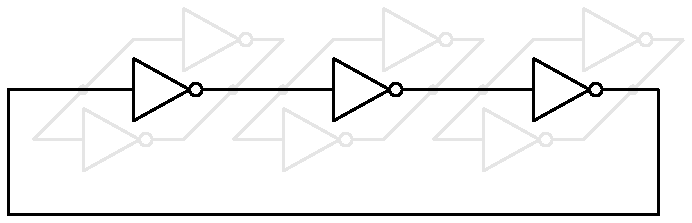
\includegraphics[width=250pt]{slike/prezentacija/ringOscillator0.pdf}
	\end{figure}
	\DCOformula           
\end{frame}
{\samenumbered
\begin{frame}{\DCO: \subsecname}
	\begin{figure}
		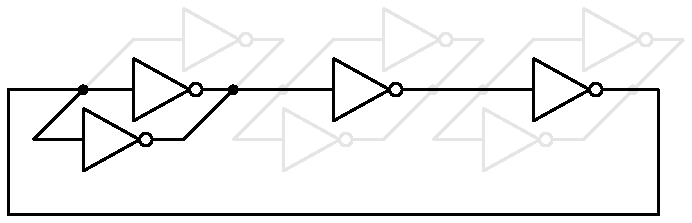
\includegraphics[width=250pt]{slike/prezentacija/ringOscillator1.pdf}
	\end{figure}
	\DCOformula  
\end{frame}}
{\samenumbered
\begin{frame}{\DCO: \subsecname}
	\begin{figure}
		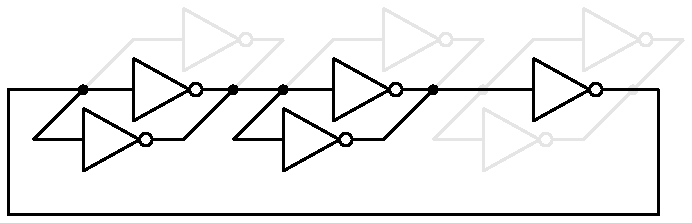
\includegraphics[width=250pt]{slike/prezentacija/ringOscillator2.pdf}
	\end{figure}
	\DCOformula 
\end{frame}}
{\samenumbered
\begin{frame}{\DCO: \subsecname}
	\begin{figure}
		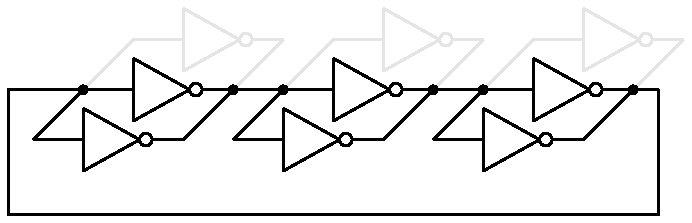
\includegraphics[width=250pt]{slike/prezentacija/ringOscillator3.pdf}
	\end{figure}
	\DCOformula
\end{frame}}
{\samenumbered
\begin{frame}{\DCO: \subsecname}
	\begin{figure}
		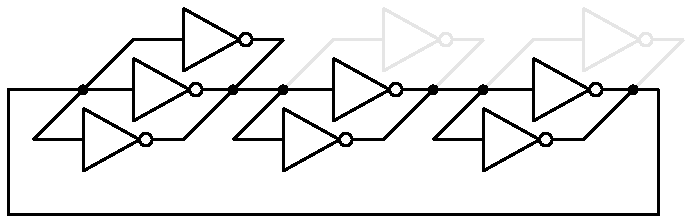
\includegraphics[width=250pt]{slike/prezentacija/ringOscillator4.pdf}
	\end{figure}
	\DCOformula
\end{frame}}
{\samenumbered
\begin{frame}{\DCO: \subsecname}
	\begin{figure}
		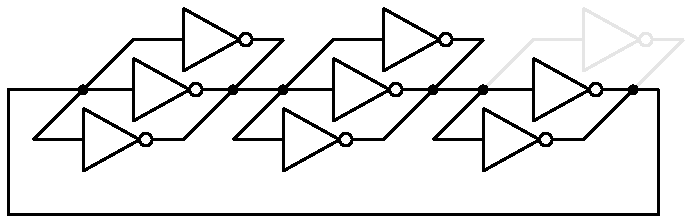
\includegraphics[width=250pt]{slike/prezentacija/ringOscillator5.pdf}
	\end{figure}
	\DCOformula
\end{frame}}
{\samenumbered
\begin{frame}{\DCO: \subsecname}
	\begin{figure}
		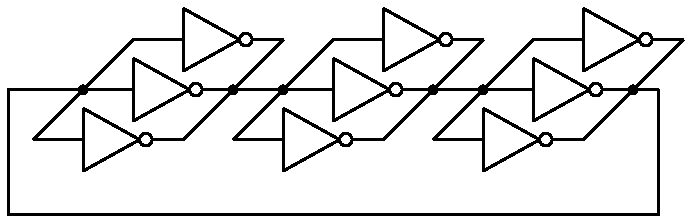
\includegraphics[width=250pt]{slike/prezentacija/ringOscillator6.pdf}
	\end{figure}
	\DCOformula
\end{frame}}

\subsection{Ћелија \DCO-a}

\begin{frame}{\DCO: \subsecname}
    \begin{columns}[t]
        \begin{column}{0.5\textwidth}
            \begin{itemize}
                \item Ћелија \DCO-a је основна градивни блок \DCO-a, који се састоји од: 
		\medskip
                \begin{enumerate}
                	\item тростатичког инвертора
                	\item И-ИЛИ управљачке јединице
                \end{enumerate}
            \end{itemize}
            \begin{figure}[!t]
	            \centering
    	        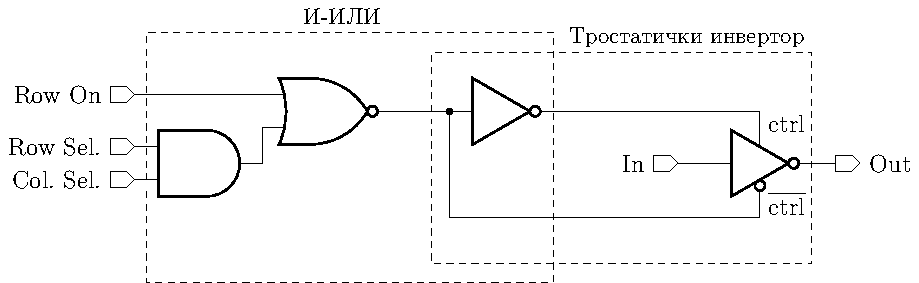
\includegraphics[scale=0.45]{slike/prezentacija/DCO_cell_circuits.pdf}
        	    \caption{Ћелија \DCO-а на нивоу логичких кола.}
            	\label{DCO_cell_circuits}
            \end{figure}
		\end{column}
		\begin{column}{0.5\textwidth}
	    \medskip
            \begin{figure}[!t]
                \centering
                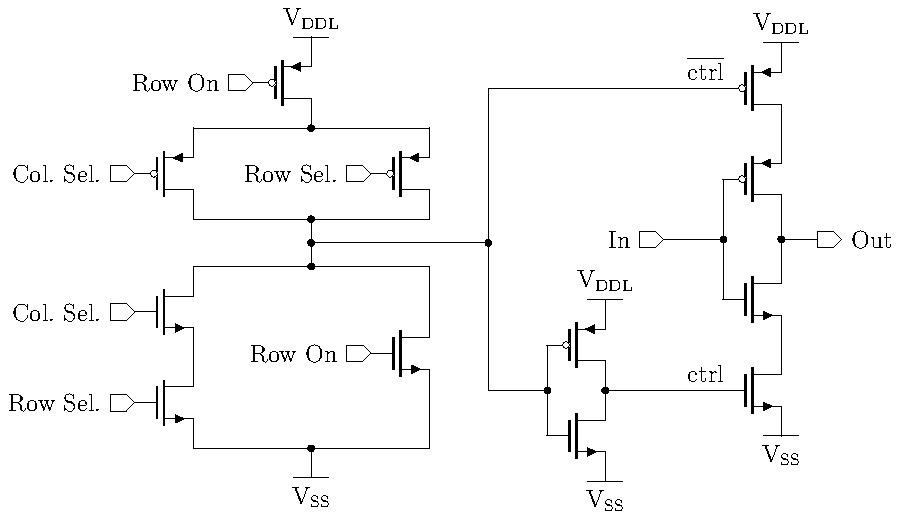
\includegraphics[scale=0.45]{slike/prezentacija/DCO_cell_transistors.pdf}
                \caption{Ћелија \DCO-а на нивоу транзистора.}
                \label{DCO_cell_transistors}
            \end{figure}
		\end{column}
	\end{columns}
\end{frame}


\subsection{Матрица ћелија \DCO-а}

\begin{frame}{\DCO: \subsecname}
	\begin{columns}[t]
        \begin{column}{0.65\linewidth}
		\vspace{-0.5cm}
        	\begin{center}
	            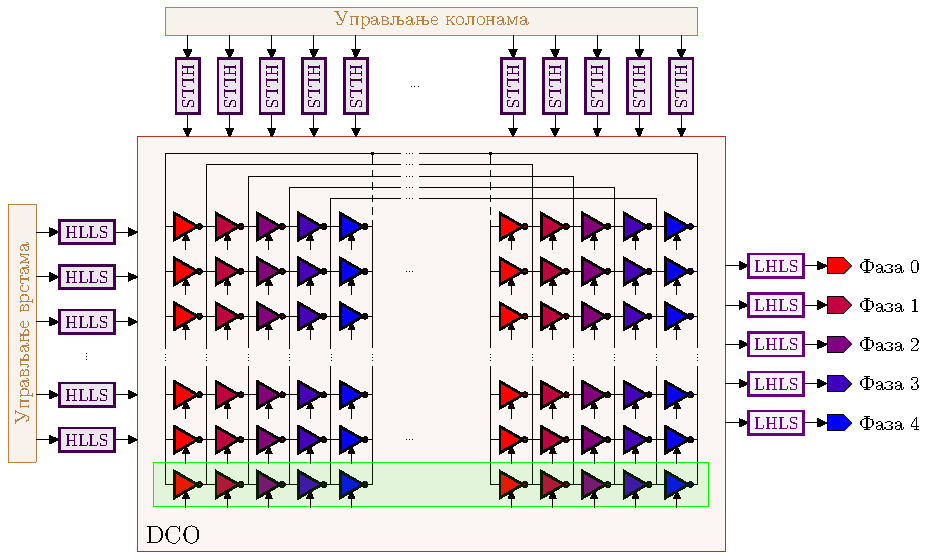
\includegraphics[scale=0.6]{slike/prezentacija/DCO.pdf} 
	        \end{center}
        \end{column}
        \begin{column}{0.35\linewidth}
		\footnotesize
        	\begin{itemize}
	        	\item петостепени прстен\\(оптималне перформансе и потрошња)
	        	\item 54 прстена (270 инвертора,\\односно ћелија \DCO-a)
	        	\item 18 врста $\times$ 15 колона\\(1 \color{green} врста увијек укључених \color {black} \\инвертора)
	        	\item 3 прстена (15 инвертора)\\по врсти
	        	\item \textbf{17$\times$15 инвертора којима \\се управља} \\ (255 корака учестаности)
	        	\item 2$\times$17+15 управљачких сигнала
	        \end{itemize}
        \end{column}
    \end{columns}    
\end{frame}

\subsection{Претварачи напонских нивоа}

\begin{frame}{\DCO: \subsecname}
    \begin{itemize}
        \item \DCO\ ради на сопственом напону напајања ($\text{V}_\text{DDL}$), а то је омогућено додавањем претварача напонских нивоа на улазе и излазе \DCO-a.
    \end{itemize}
    \vspace{-0.5cm}
    \begin{columns}[t]
        \begin{column}{0.5\textwidth}
            \begin{figure}[!h]
	    \medskip
            \centering
            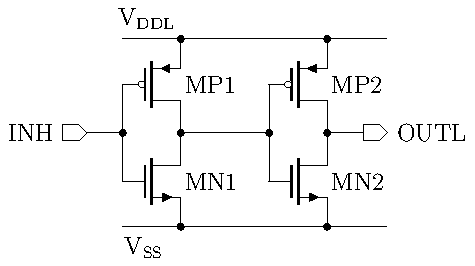
\includegraphics[scale=0.65]{slike/prezentacija/Level_shifter_HL.pdf}
            \caption{Претварач са високог на низак напонски ниво.}
            \label{Level_shifter_HL}
            \end{figure}
		\end{column}
		\begin{column}{0.5\textwidth}
            \begin{figure}[!h]
                \centering
                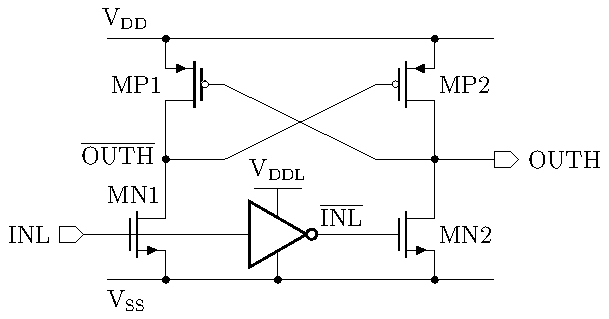
\includegraphics[scale=0.65]{slike/prezentacija/Level_shifter_LH.pdf}
                \caption{Претварач са ниског на висок напонски ниво.}
                \label{Level_shifter_LH}
            \end{figure}
		\end{column}
	\end{columns}
    \begin{itemize}
        \item Тиме је омогућено независно подешавање напона напајања \DCO-a након фабрикације, да би се постигао жељени опсег и корак учестаности и смањила потрошња снаге. % (quadratic dependence on the supply voltage)
    \end{itemize}	
\end{frame}

\section{Управљачка логика}
\begin{frame}{\secname}
\centering
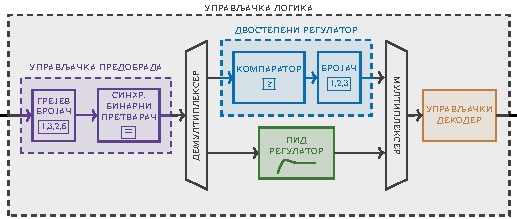
\includegraphics[scale=1]{slike/prezentacija/FLL_CTRL.pdf} 
\medskip
\begin{itemize}
	\item Управљачка предобрада
	\item Двостепени регулатор / \PID\ регулатор
	\item Управљачки декодер
\end{itemize}
\end{frame}

\subsection{Управљачка предобрада}

\begin{frame}{\secname: \subsecname}
	\vspace{-0.5cm}
	\begin{columns}[t]
        \begin{column}{0.25\linewidth}
        	\begin{center}
        		\vspace{-0.2cm}
	            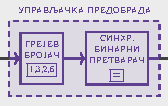
\includegraphics[scale=1.3]{slike/prezentacija/CTRL_PREPROC.pdf} 
	        \end{center}
        \end{column}
        \begin{column}{0.75\linewidth}
        	\begin{center}
			\vspace{-0.3cm}
            	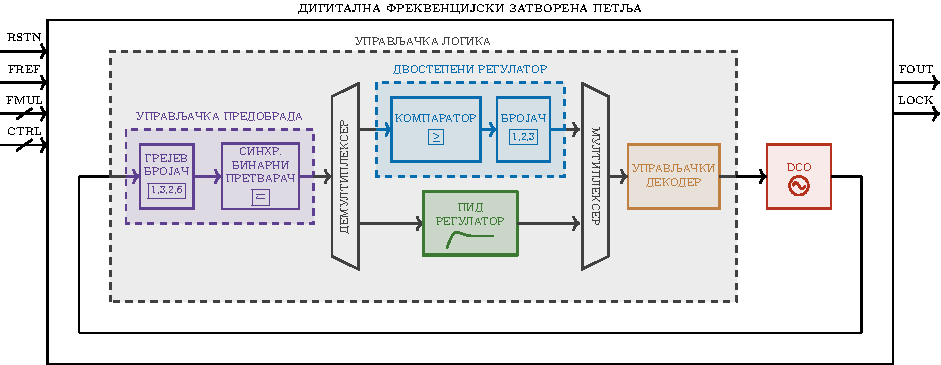
\includegraphics[scale=0.5]{slike/prezentacija/FLL.pdf}
            \end{center}
        \end{column}
    \end{columns}
    \medskip
	\begin{itemize}
		\item Претвара учестаност такта \DCO-а у бинарну вриједност управљачке логике помоћу:
		\begin{enumerate}
			\color{\CtrlPreprocColor}
			\item Грејевог бројача: броји периоде такта \DCO-а унутар периода референтног такта
			\item Синхронизатора и бинарног конвертора: омогућавају исправно пребацивање вриједности Грејевог бројача из области такта \DCO-a у област референтног такта и претварање у бинарни код.
		\end{enumerate}
		\smallskip
	\item У Грејевом коду свака узастопна вриједност се разликује за по један бит. Заједно са синхронизатором који се састоји од два флип-флопа, \underline{ризик од ефеката метастабилности је значајно смањен}.
	\end{itemize}
\end{frame}

\subsubsection{Синхронизатор}

\begin{frame}{\secname: \subsecname (\subsubsecname)}
	\centering
	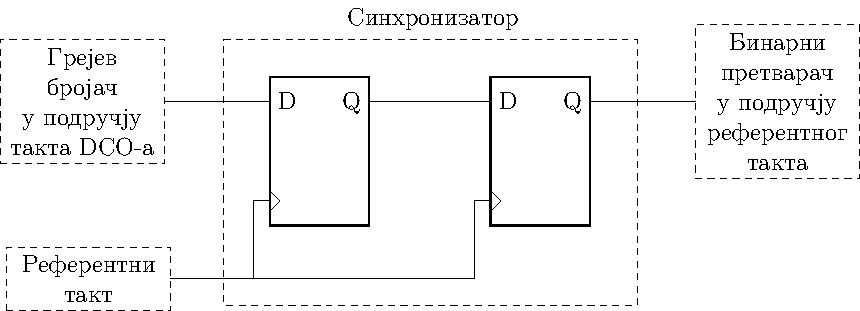
\includegraphics[scale=0.9]{slike/prezentacija/syncronizer.pdf}
\end{frame}

\subsection{Двостепени регулатор}

\begin{frame}{\secname: \subsecname}
	\vspace{-0.6cm}
	\begin{columns}[t]
        \begin{column}{0.25\linewidth}
        	\begin{center}
        		\vspace{-0.2cm}
	            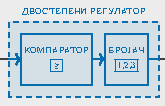
\includegraphics[scale=1.3]{slike/prezentacija/BB_CTRL.pdf} 
	        \end{center}
        \end{column}
        \begin{column}{0.75\linewidth}
        	\begin{center}
            	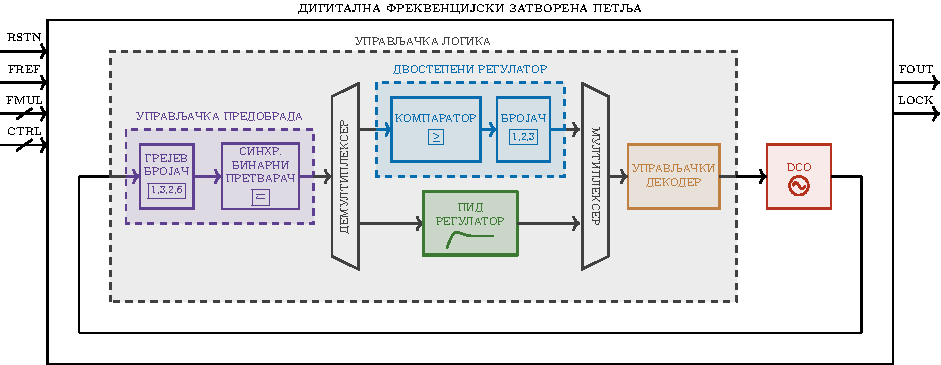
\includegraphics[scale=0.5]{slike/prezentacija/FLL.pdf}
            \end{center}
        \end{column}
    \end{columns}
    \medskip	
	\begin{itemize}
		\item Двостепени (или on-off) регулатор има три стања: инкрементирај, декрементирај и онемогући наредни блок.
		\smallskip		
		\item Састоји се од два блока:
		\begin{itemize}		
			\color{\BBctrlColor}
			\item Компаратор: упоређује улазни умножак учестаности са узоркованом вриједношћу бројача такта \DCO-a и шаље сигнал инкрементирања, декрементирања или онемогућавања наредном блоку.
			\item Двосмјерни бројач: бинарни бројач који директно утиче на улазну управљачку вриједност \DCO-a.
		\end{itemize}
		\smallskip
		 % \pause
		\item Осигурава се управљање учестаношћу корак по корак и њено коначно закључавање.
	\end{itemize}
\end{frame}

\subsection{\PID\ регулатор}

\begin{frame}{\secname: \subsecname}
	\vspace{-0.6cm}
	\begin{columns}[t]
        \begin{column}{0.25\linewidth}
        	\begin{center}
	        	\vspace{0.4cm}
	            
\includegraphics[scale=1.82]{slike/prezentacija/PID_CTRL.pdf} 
	        \end{center}
        \end{column}
        \begin{column}{0.75\linewidth}
        	\begin{center}
            	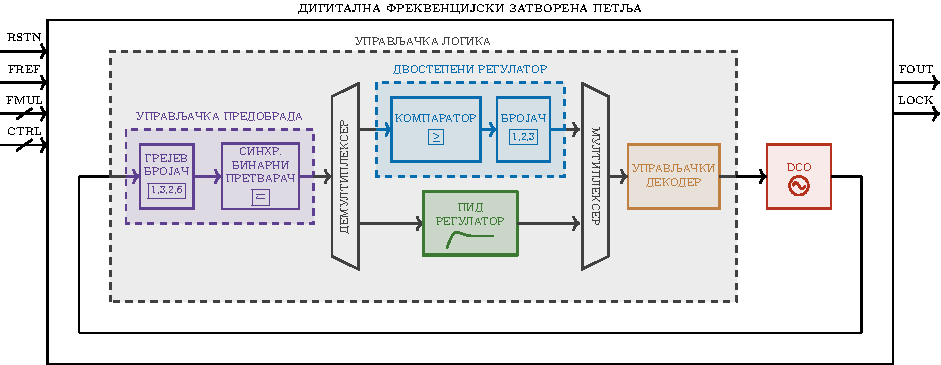
\includegraphics[scale=0.5]{slike/prezentacija/FLL.pdf}
            \end{center}
        \end{column}
    \end{columns}
    \medskip
	\begin{itemize}
		\item \PID\ регулатор је повратни управљачки механизам, који константно скалира и исправља сигнал грешке (која у овдје представља разлику између узорковане вриједности бројача такта \DCO-а и улазног умношка учестаности):
		\begin{itemize}
			\color{\PIDctrlColor}
			\item П компонента: контролише брзину одзива система
			%, by directly multiplying the error signal by a constant factor.
			\item И компонента: смањује грешку стационарног стања
			%, by scaling the error by a constant factor and summing the result over time.
			\item Д компоненета: ограничава излаз да би се смањило потенцијално прекорачење или осцилације. 
			% caused by the P and I components, without decreasing the controller speed It is proportional to the error change rate.
		\end{itemize}
		\smallskip
		\item Како је умножак учестаности константан и нема наглих промјена на улазу, П и И компоненте су довољне за гладак и стабилан одзив система.
	\end{itemize}
\end{frame}

\begin{frame}{\secname: \subsecname}
	\centering
	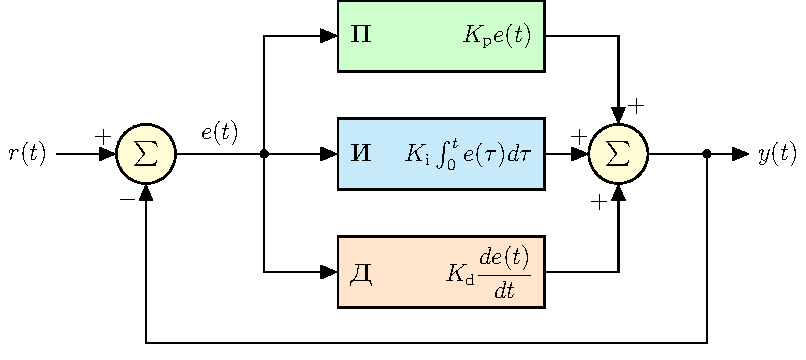
\includegraphics[scale=0.8]{slike/prezentacija/pid.pdf}
	\begin{equation}
		y(t)= K_\text{p}e(t) + K_\text{i}\int_{0}^{t}e(\tau)d\tau + K_\text{d}\frac{de(t)}{dt} \nonumber
	\end{equation}
\end{frame}

\subsection{Управљачки декодер}

\begin{frame}{\secname: \subsecname}
	\vspace{-0.6cm}
	\begin{columns}[t]
        \begin{column}{0.25\linewidth}
            \begin{center}
		    \vspace{0.4cm}
	        
\includegraphics[scale=2.1]{slike/prezentacija/CTRL_DEC.pdf} 
	    \end{center}
        \end{column}
        \begin{column}{0.75\linewidth}
        	\begin{center}
            	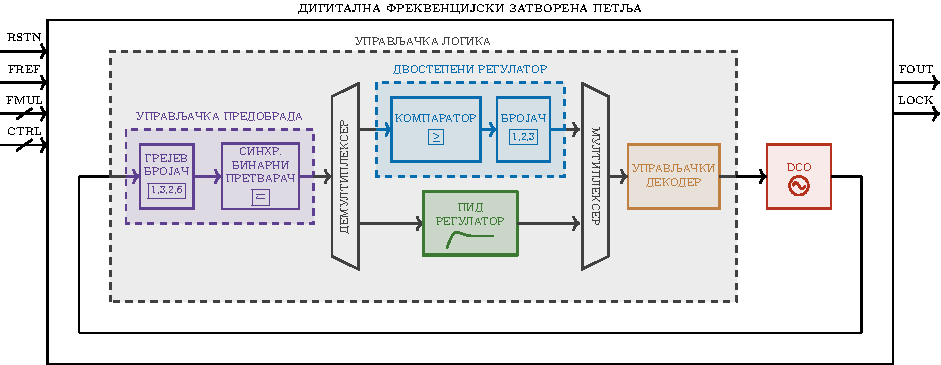
\includegraphics[scale=0.5]{slike/prezentacija/FLL.pdf}
            \end{center}
        \end{column}
    \end{columns}
    \medskip
	\begin{itemize}
		\item Претвара управљачки податак из једне бинарне вриједности у скуп управљачких улаза \DCO-а:
        \begin{itemize}
		\color{\CtrlDecColor}
		\item \textsl{Row On}: унарни вектор, који укључује само читаве врсте тростатичких инвертора.
		\item \textsl{Row Select}: један од $n$ вектор, који укључује једну додатну врсту торстатичких инвертора.
		\item \textsl{Column Select}: унарни вектор, који може да укључује колоне тростатичких инвертора.
		\end{itemize}
		\smallskip
	\item Да би тростатички инвертор био укључен потребно је да или \textsl{Row On}, или и \textsl{Row Select} и \textsl{Column Select} за одговарајући бит имају логичку вриједност 1.% (управљачка јединица из ћелије \DCO-a).
	\end{itemize}
\end{frame}

\begin{frame}{\secname: \subsecname}
	\centering
	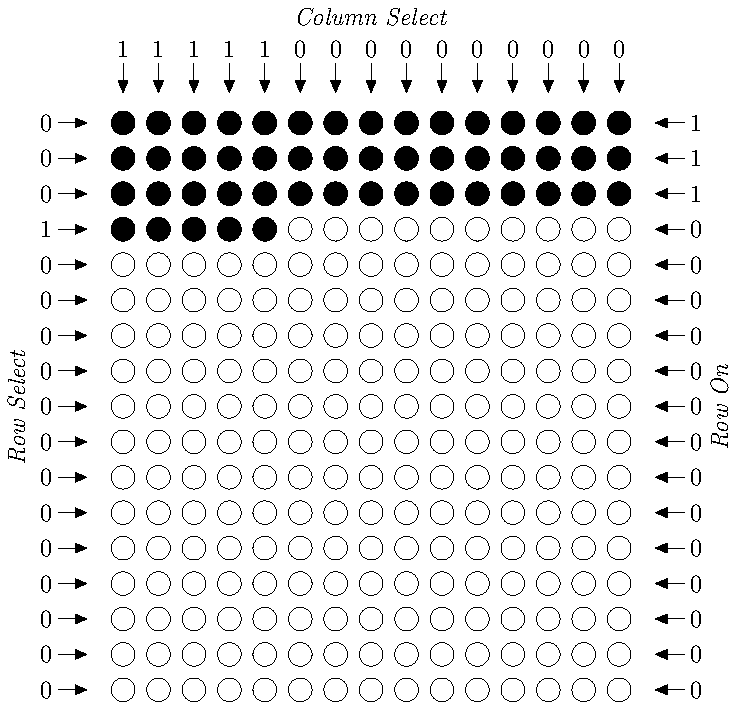
\includegraphics[scale=0.6]{slike/prezentacija/ctrl_dec_example.pdf}
\end{frame}

\section{Имплементација и резултати симулација}

\begin{frame}{\secname}
	\begin{itemize}
		\item \FLL\ је имплементиран коришћењем SystemVerilog језика за опис хардвера, у 130\,nm CMOS технологији.
		\smallskip
		\item \DCO\ је имплементиран као посебна компонента коришћењем библиотеке стандардних ћелија. 
		\smallskip
		\item FREF=16\,MHz, FMUL=40 $\implies$ FOUT=640\,MHz, FRES=2,8\,MHz.
		\smallskip
		\item $\text{V}_\text{DD}$=1,2\,V, $\text{V}_\text{DDL}$=1,1\,V, $\text{I}_\text{DD}$=0,9\,mA, $\text{I}_\text{DDL}$=2,185\,mA, $\implies$ $\text{P}_\text{FLL}$=3,5\,mW		
		\smallskip
		\item Читав дизајн заузима око 33000\,\text\textmu m$^\text2$, од чега око 13\,\% заузима \DCO\ (доле десно у приказаном лејауту \FLL-а):
		\medskip
	   	\begin{figure}[!h]
  	    	    \centering
        	    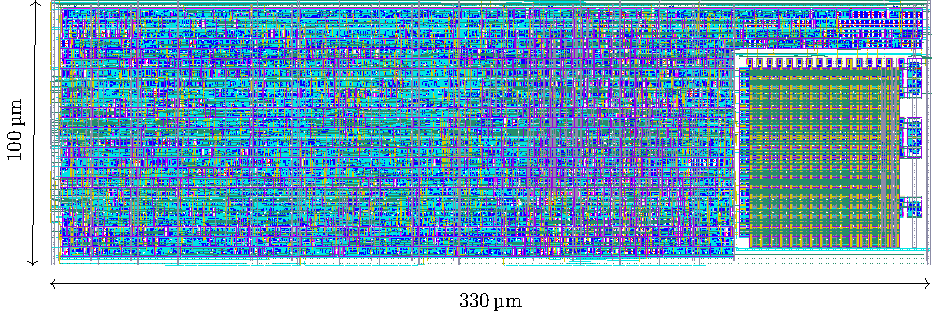
\includegraphics[scale=0.7]{slike/prezentacija/layout_FLL.pdf}
    	        \end{figure}		
	\end{itemize}
\end{frame}

\subsection{Лејаут \DCO-a}

\begin{frame}{\secname: \subsecname}
	\begin{figure}[!h]
  		\centering
        	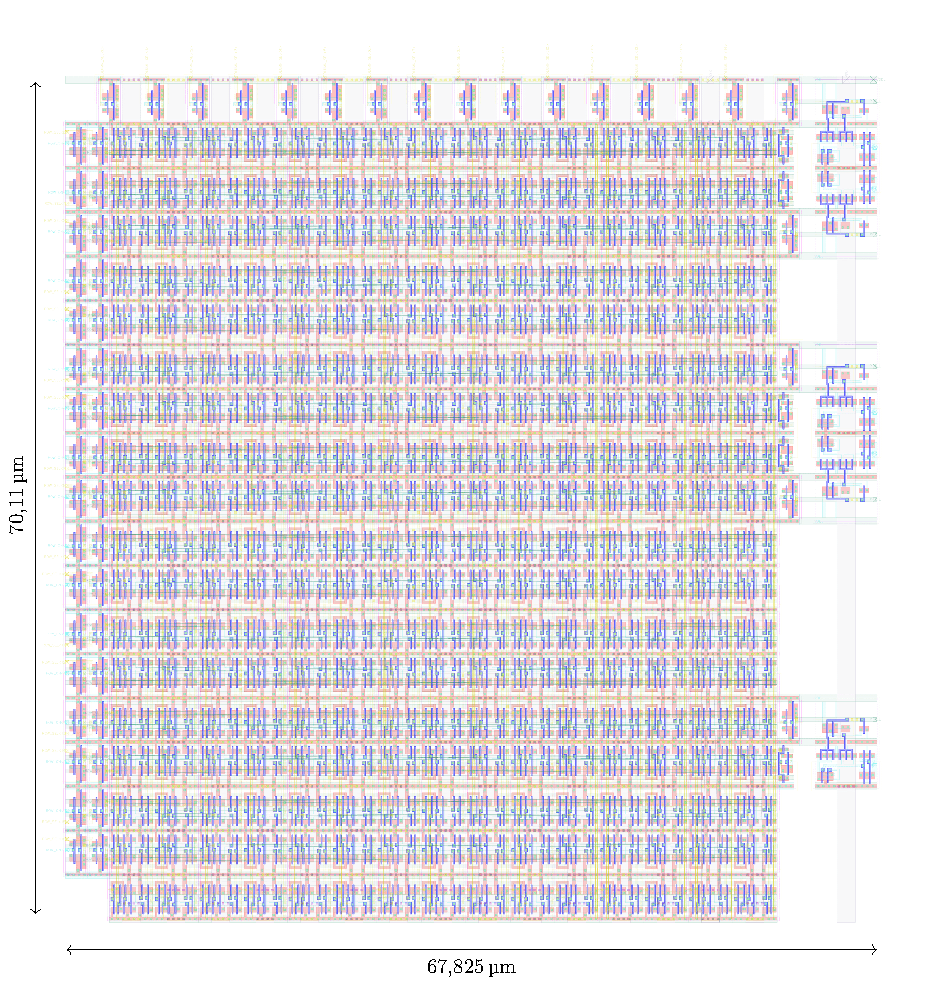
\includegraphics[scale=0.45]{slike/prezentacija/layout_dco5_hl_lh_130.pdf}
    	\end{figure}		
\end{frame}

\begin{frame}{\secname: \subsecname}
	\begin{columns}[t]
        \begin{column}{0.6\linewidth}
	\vspace{-0.7cm}
	\begin{figure}[!h]
  		\centering
		\begin{tikzpicture}
	 	% The image node
        	\node[inner sep=0] (layout_dco5_130) { 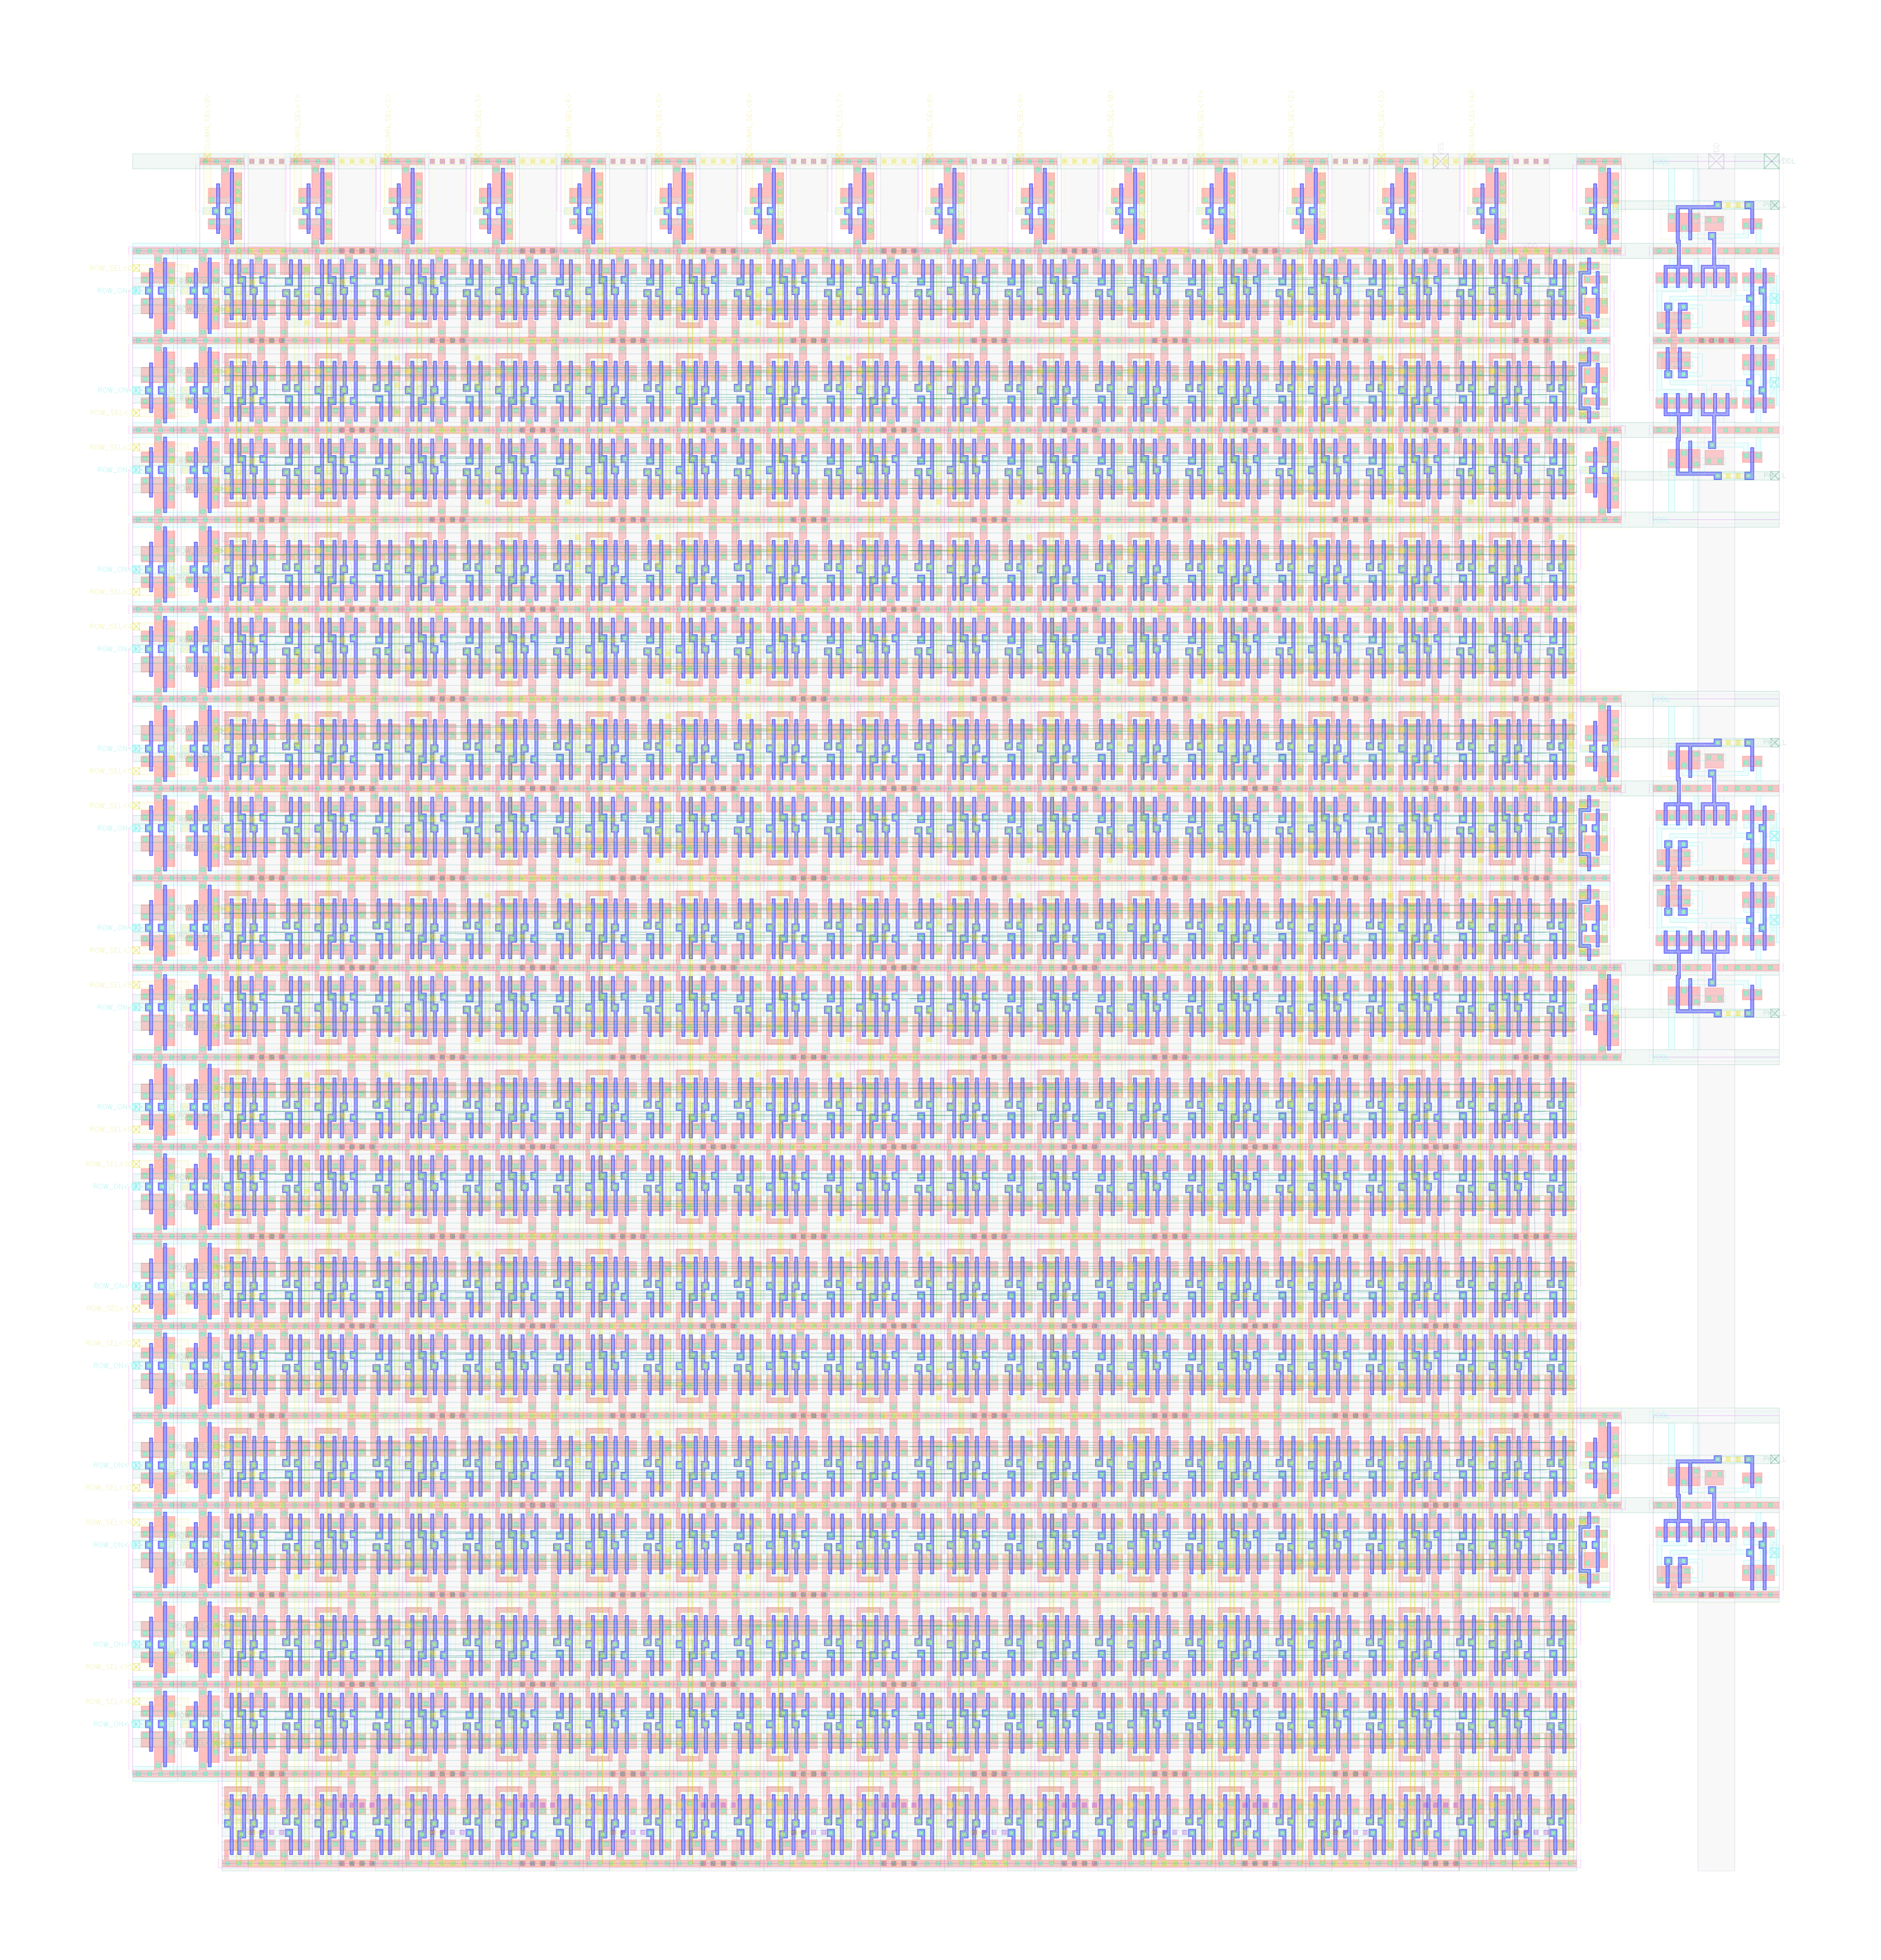
\includegraphics[scale=0.072]{slike/prezentacija/layout_dco5_hl_lh_130.png} };
		\draw[thick, red] (-2.85,2.9) --++ (5.4,0) --++ (0,-6.5) -|++ (-5.4,6.5);
		\draw[thick, OliveGreen] (-2.82,2.94) --++ (5.4,0) --++ (0,0.35) --++ (-5.8,0) --++ (0,-6.5) --++ (0.34,0) --++ (0,6.15) --++ (0.1,0);
		\draw[thick, blue] (2.82,3.3) --++ (0.6,0) --++ (0,-6) -|++ (-0.6,6);
        	\end{tikzpicture}
    	\end{figure}		
        \end{column}
        \begin{column}{0.4\linewidth}
		\bigskip
		\bigskip
		\begin{itemize}
			\item \color{red} Матрица ћелија \DCO-а
			\bigskip
			\item \color{OliveGreen} Претварачи са високог на низак напонски ниво
			\bigskip
			\item \color{blue} Претварачи са ниског на висок напонски ниво
		\end{itemize}
        \end{column}
    \end{columns}
\end{frame}

\subsection{Лејаут ћелије \DCO-a}

\begin{frame}{\secname: \subsecname}
	\begin{figure}[!h]
  		\centering
		\begin{tikzpicture}
	 	% The image node
		\begin{scope}[shift={(0,0)}, name=DCO5]
        	\node[inner sep=0] (layout_dco5_130) { 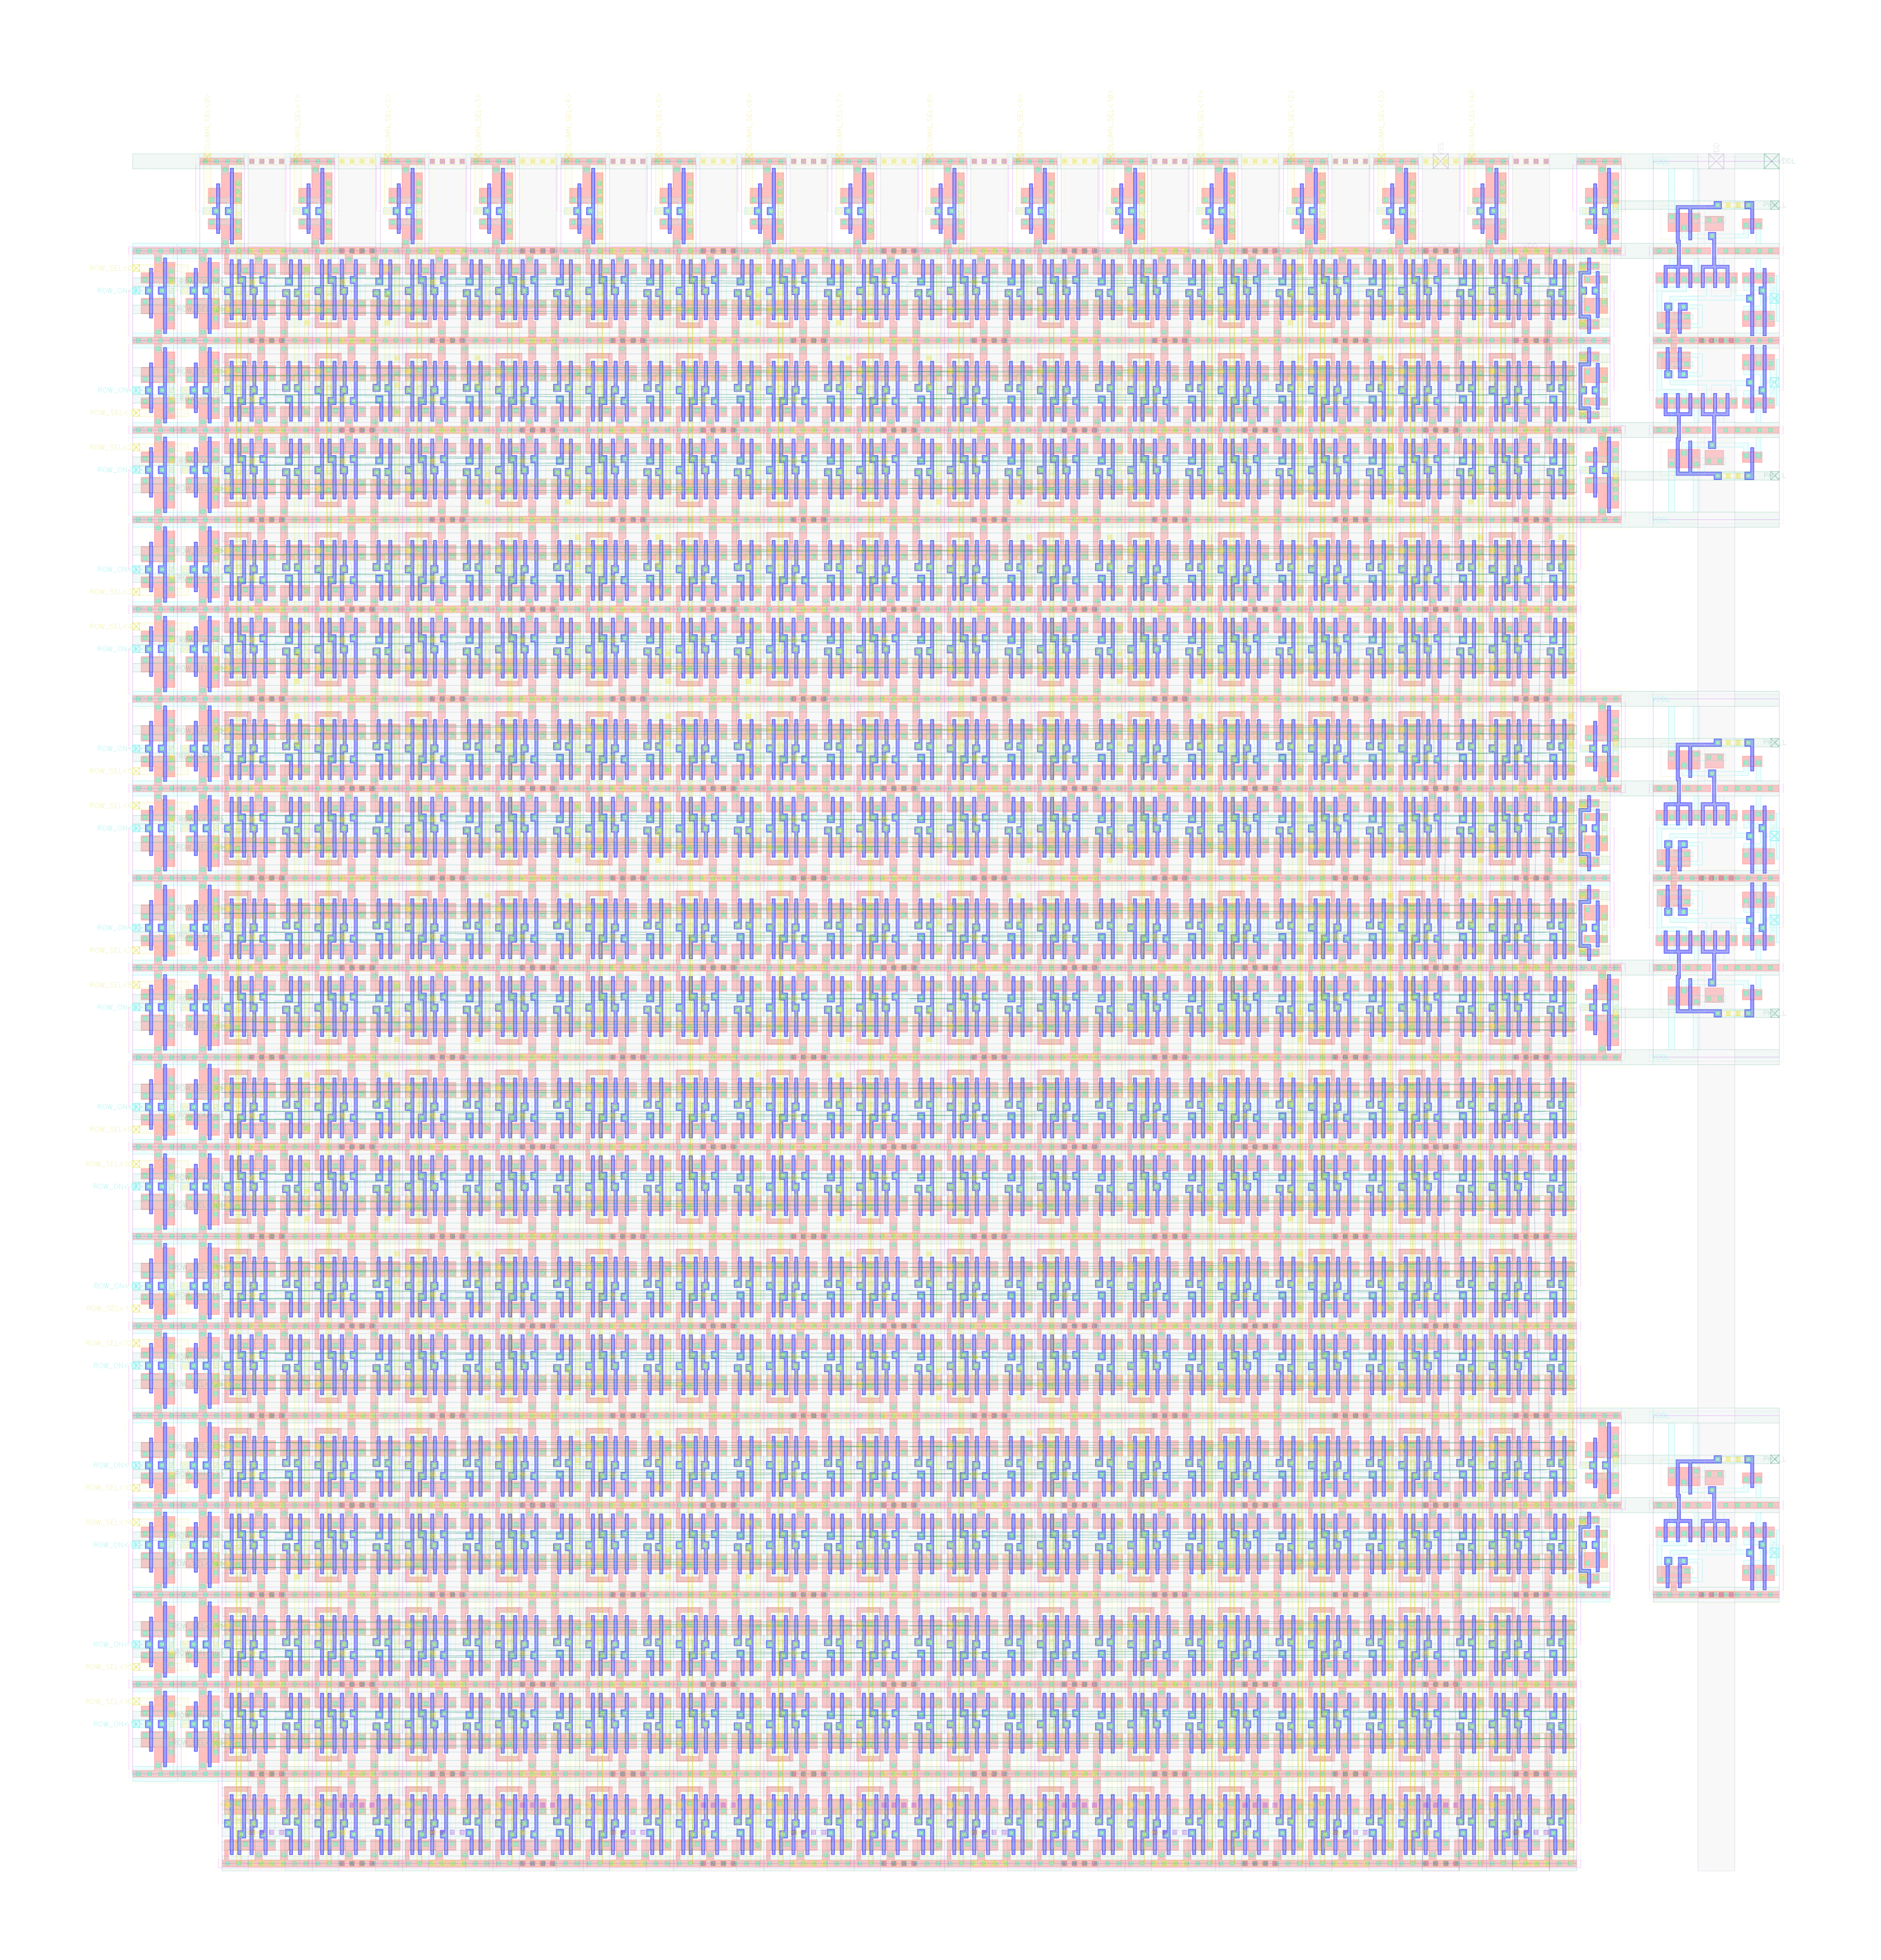
\includegraphics[scale=0.07]{slike/prezentacija/layout_dco5_hl_lh_130.png} };
		\end{scope}
		\begin{scope}[shift={(7.4,0)}, name=DCO_cell]
        	\node[inner sep=0] (layout_dco_cell) { 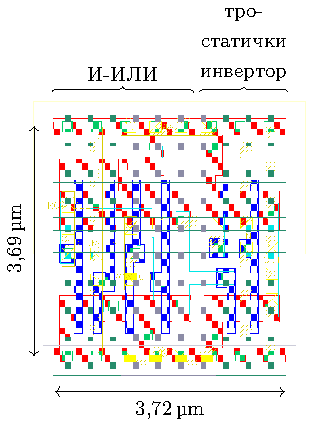
\includegraphics[scale=0.9]{slike/prezentacija/layout_dco_cell.pdf} };
		\end{scope}
		\draw[thick, red] (1.06,0.05) --++ (0.36,0) --++ (0,0.35) -|++ (-0.36,-0.35) ;
		\draw[->, dashed, thick, red] (1.42,0.2) --++ (3.4,0);
		\draw[thick, red] (4.82, -3.3) --++ (0,6.7) --++ (5,0) |-++ (-5,-6.7);
        	\end{tikzpicture}
    	\end{figure}		
\end{frame}

\subsection{Лејаут HL претварача}

\begin{frame}{\secname: \subsecname}
	\begin{figure}[!h]
  		\centering
		\begin{tikzpicture}
	 	% The image node
		\begin{scope}[shift={(0,0)}, name=DCO5]
        	\node[inner sep=0] (layout_dco5_130) { 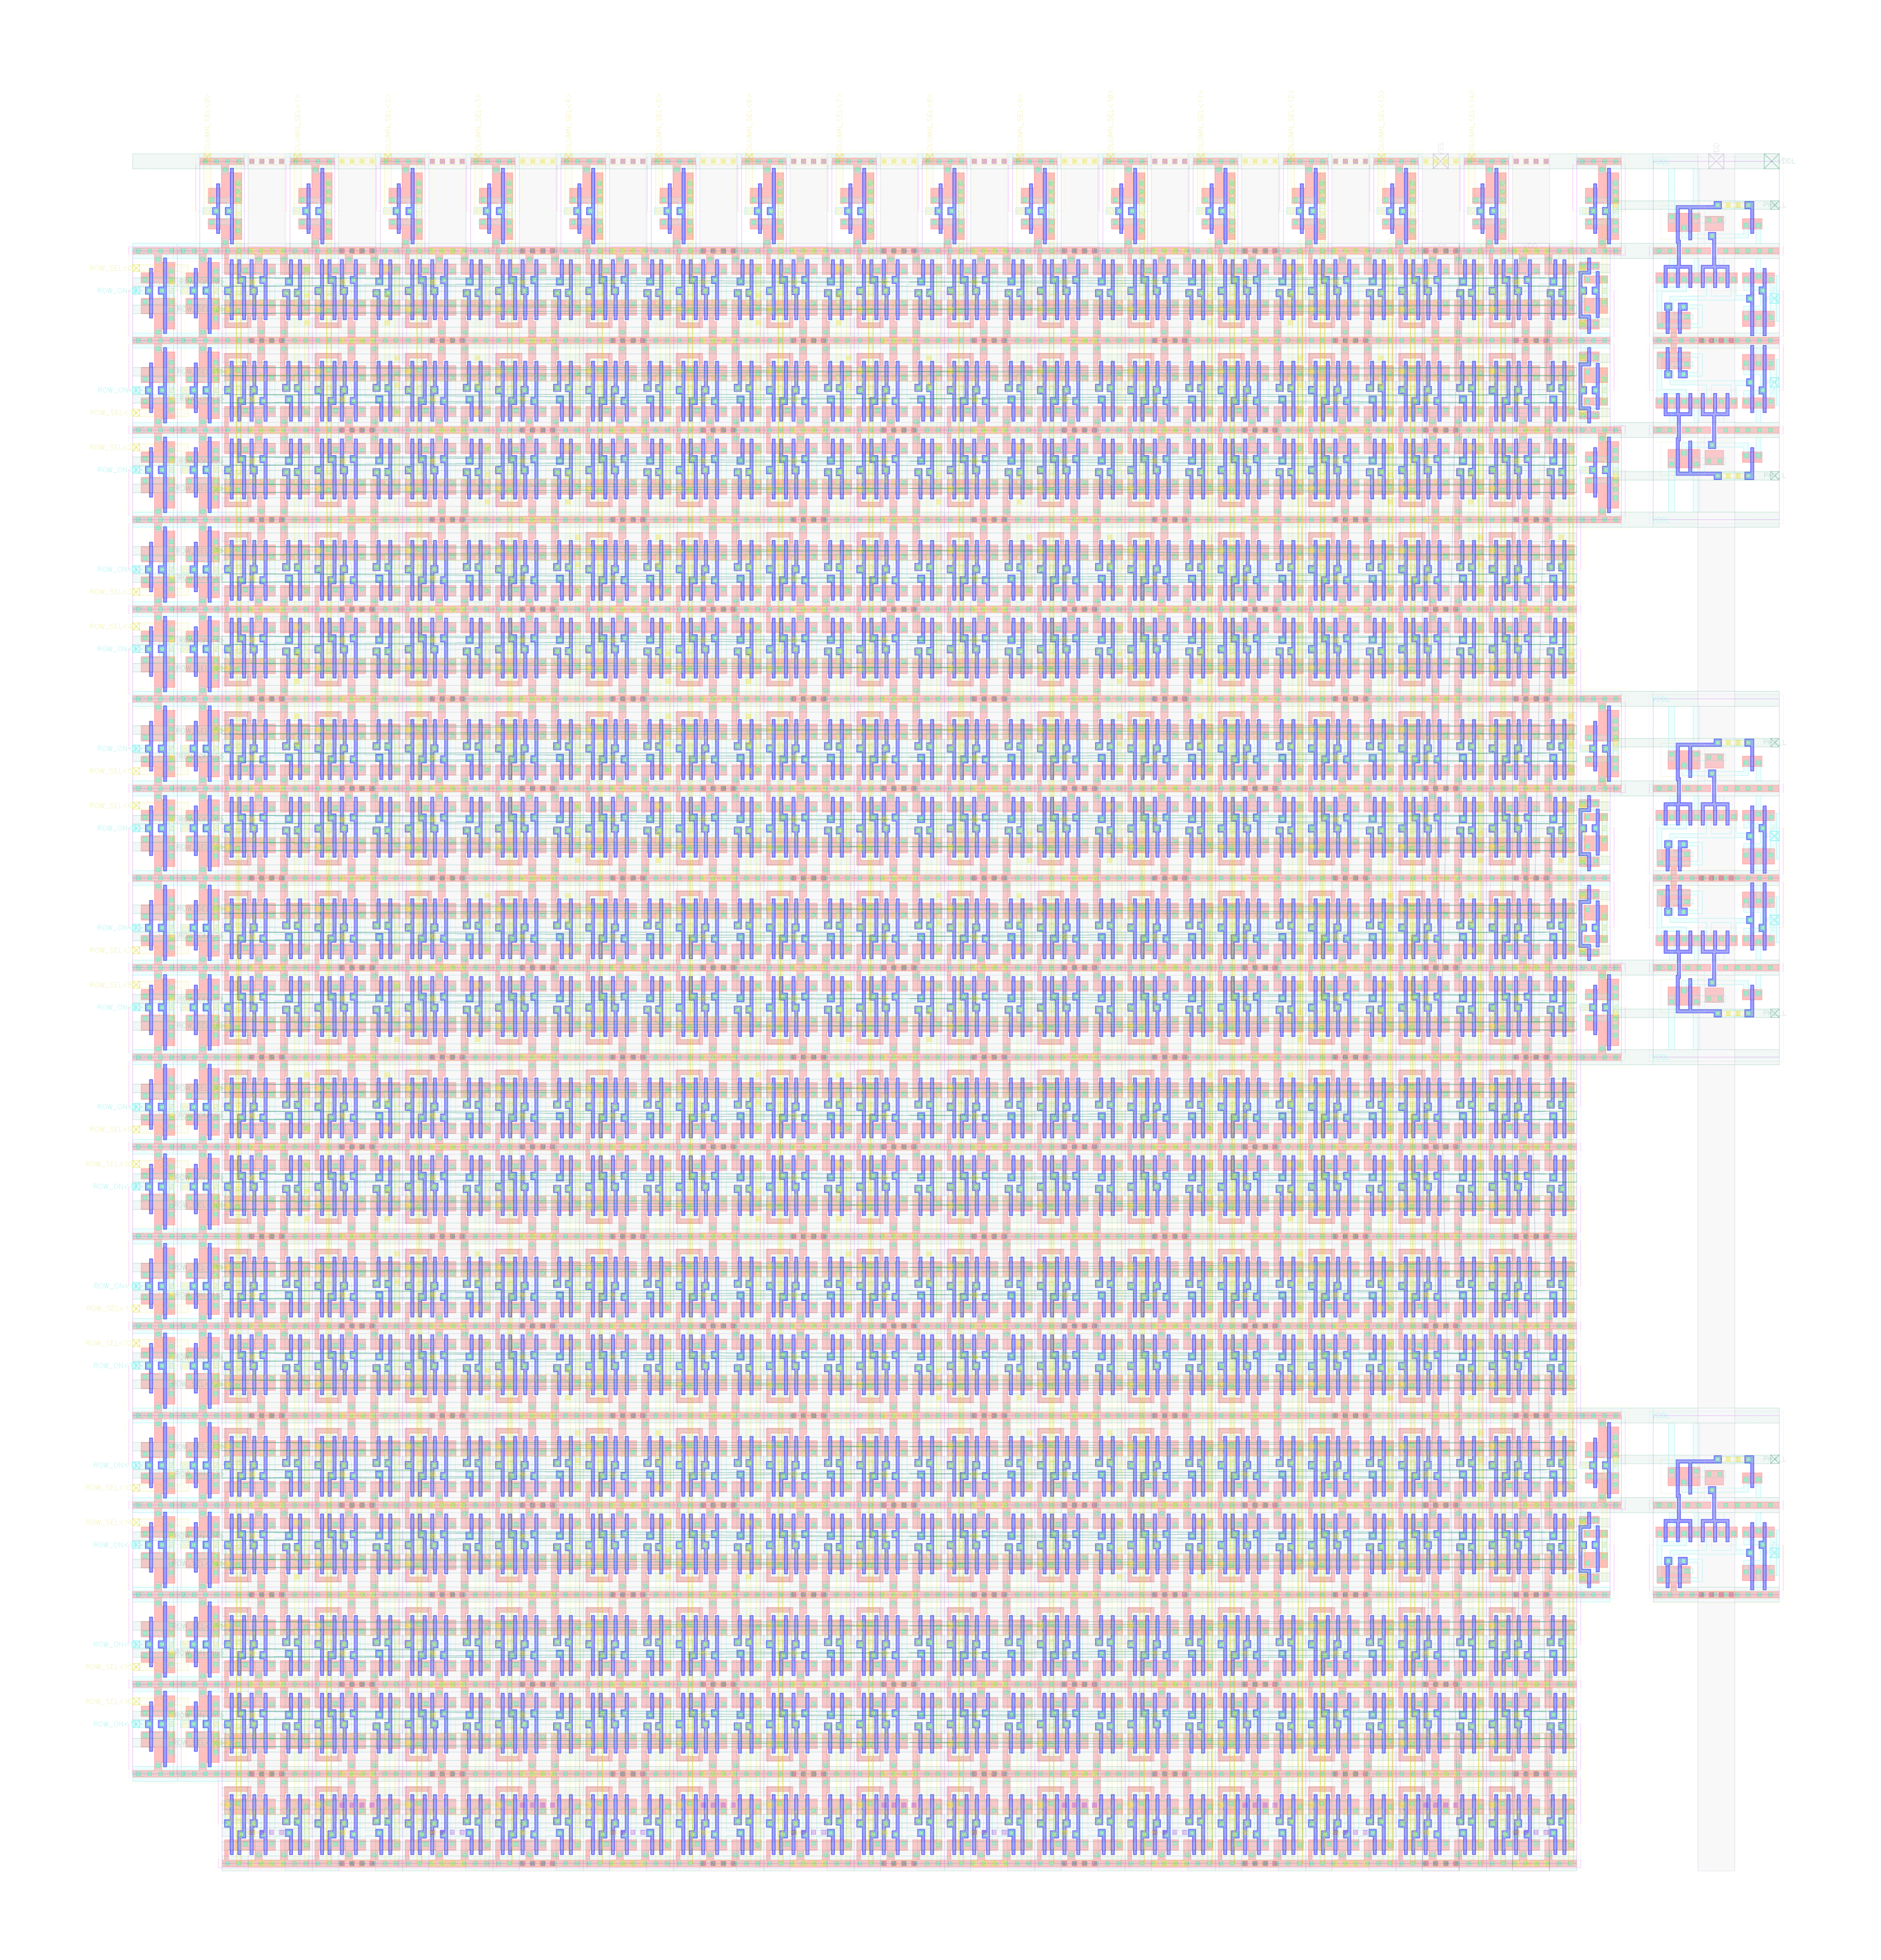
\includegraphics[scale=0.07]{slike/prezentacija/layout_dco5_hl_lh_130.png} };
		\end{scope}
		\begin{scope}[shift={(7.4,0)}, name=lvl_hl]
        	\node[inner sep=0] (layout_lvl_hl) { 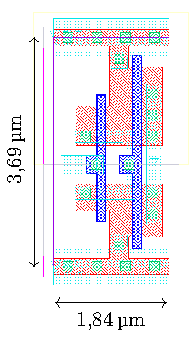
\includegraphics[scale=0.9]{slike/prezentacija/layout_lvl_hl.pdf} };
		\end{scope}
		\draw[thick, red] (-3.15,0.05) --++ (0.19,0) --++ (0,0.35) -|++ (-0.19,-0.35) ;
		\draw[->, dashed, thick, red] (-2.96,0.2) --++ (8.5,0);
		\draw[thick, red] (5.54, -2.8) --++ (0,5.5) --++ (3.5,0) |-++ (-3.5,-5.5);
        	\end{tikzpicture}
    	\end{figure}		
\end{frame}

\subsection{Лејаут LH претварача}

\begin{frame}{\secname: \subsecname}
	\vspace{-0.7cm}
	\begin{figure}[!h]
  		\centering
		\begin{tikzpicture}
	 	% The image node
		\begin{scope}[shift={(0,0)}, name=DCO5]
        	\node[inner sep=0] (layout_dco5_130) { 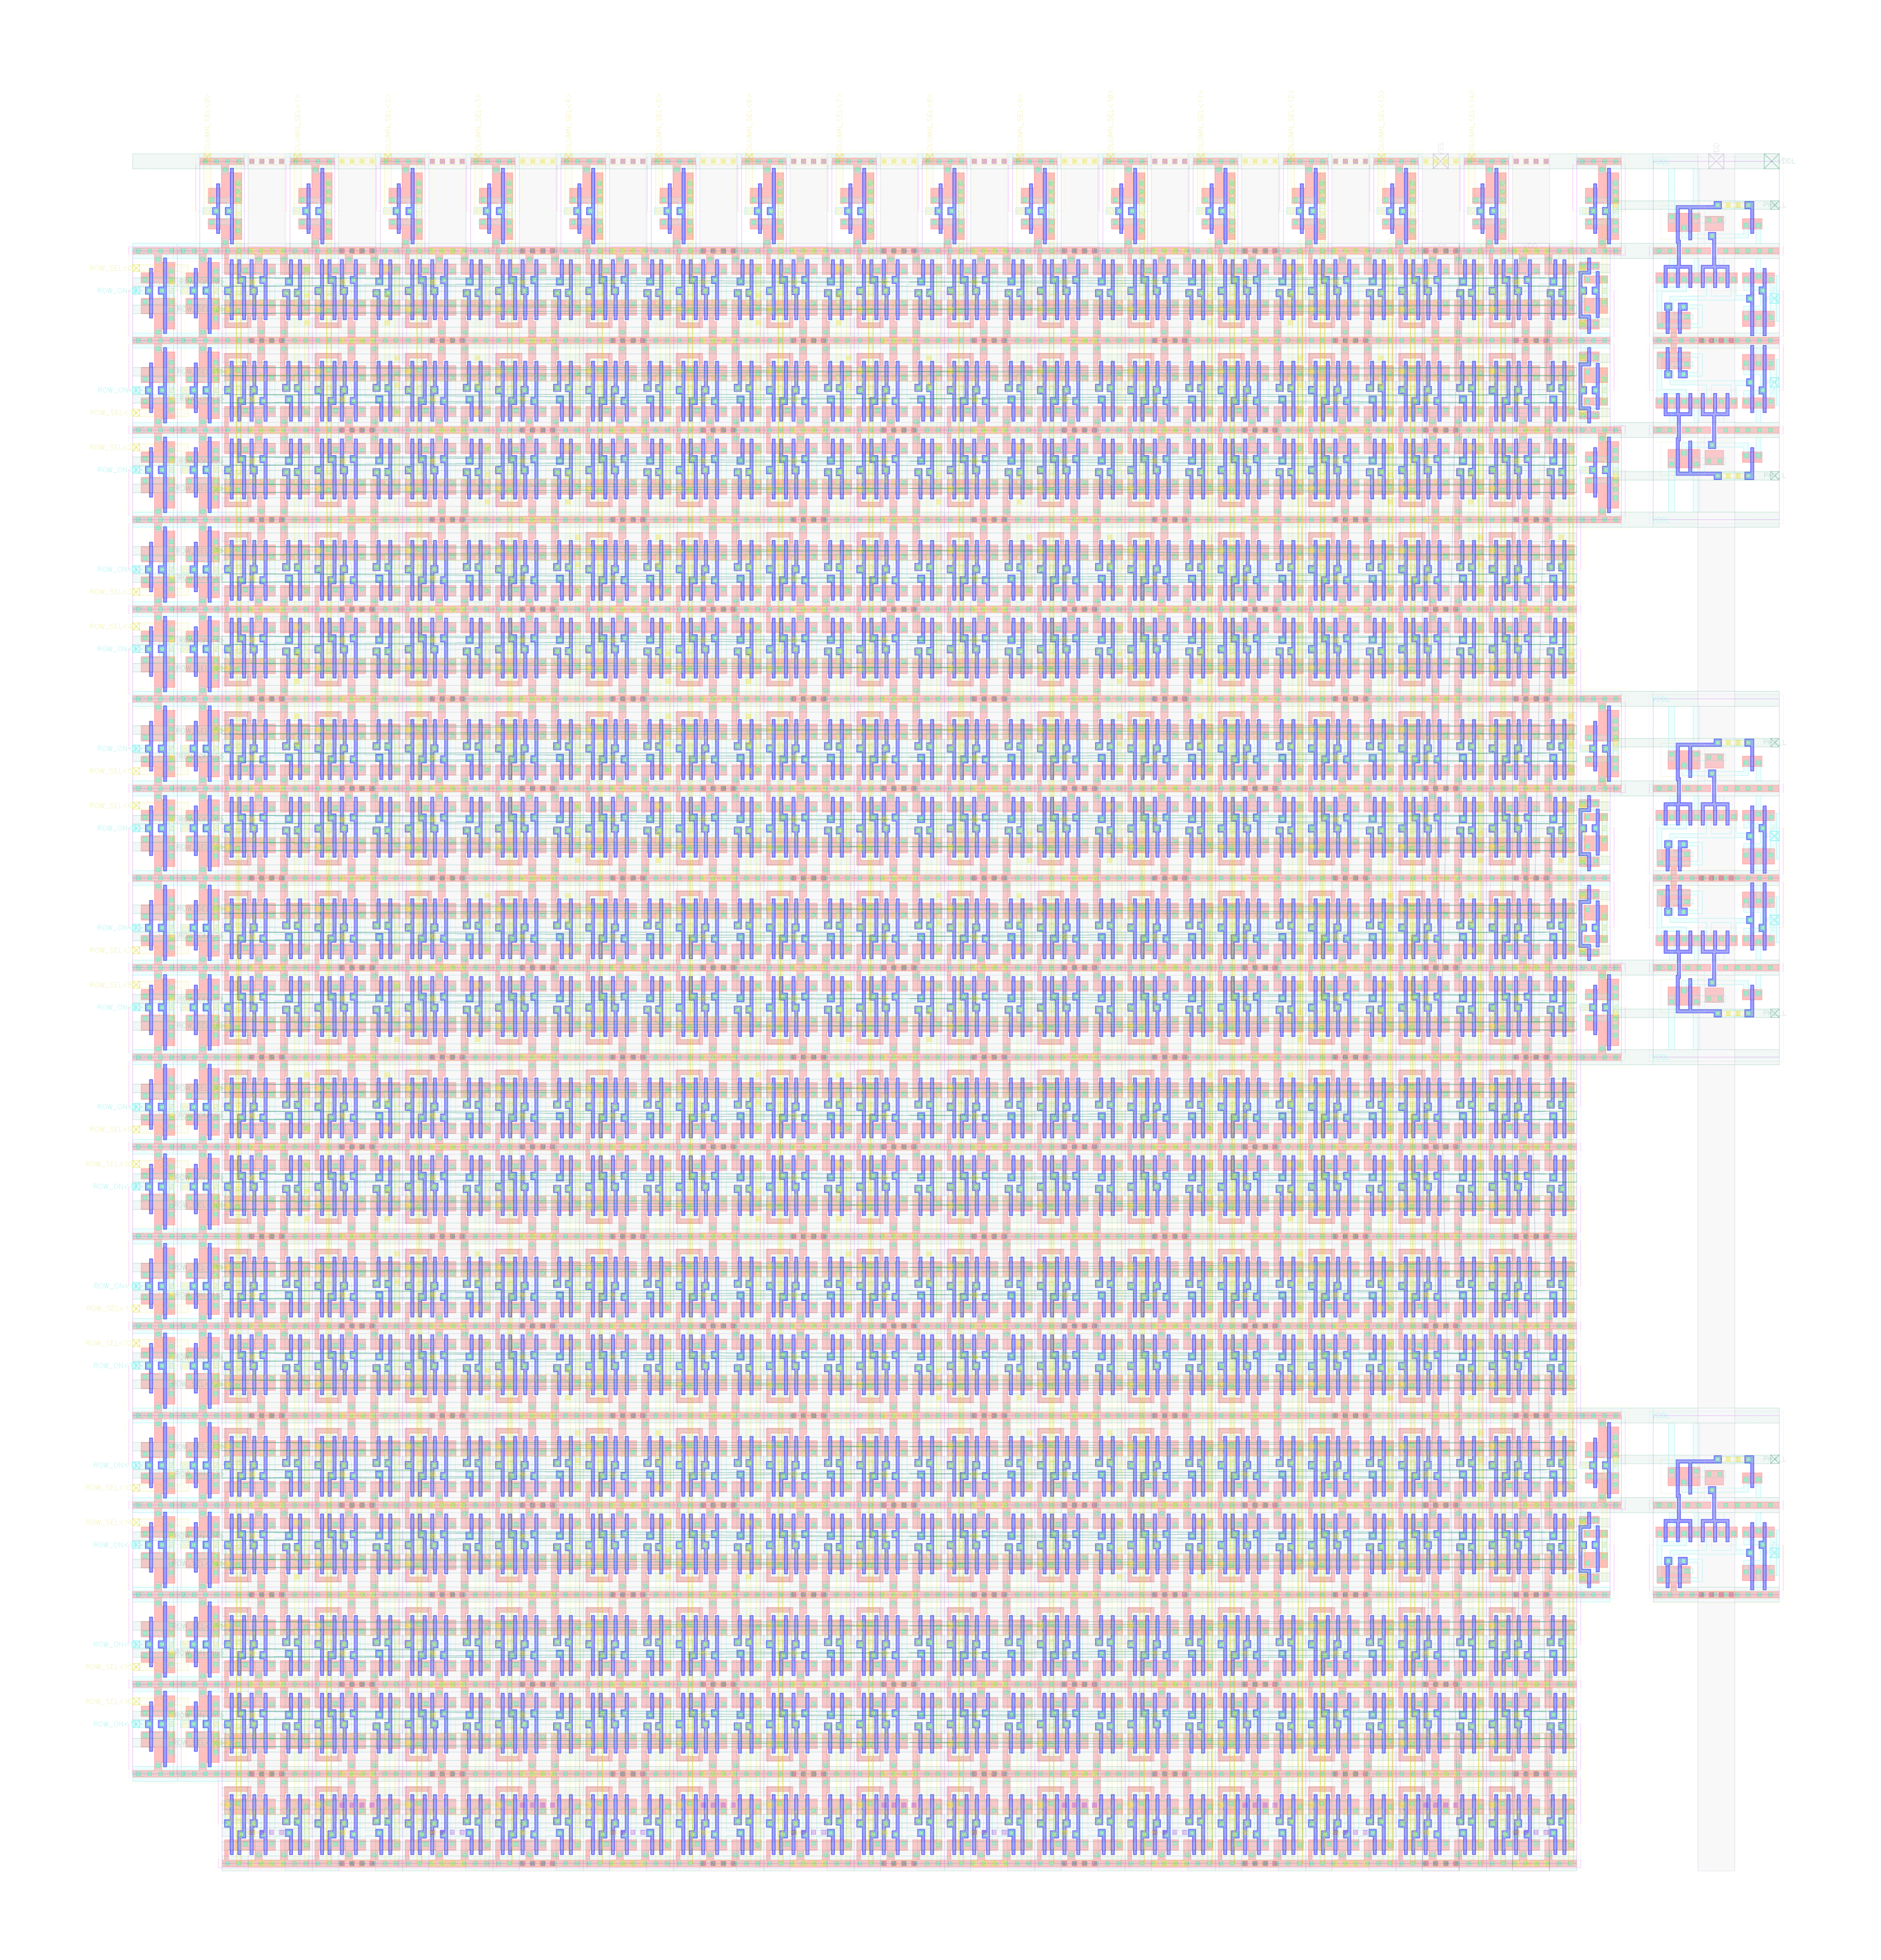
\includegraphics[scale=0.07]{slike/prezentacija/layout_dco5_hl_lh_130.png} };
		\end{scope}
		\begin{scope}[shift={(7.7,0)}, name=lvl_lh]
        	\node[inner sep=0] (layout_lvl_lh) { 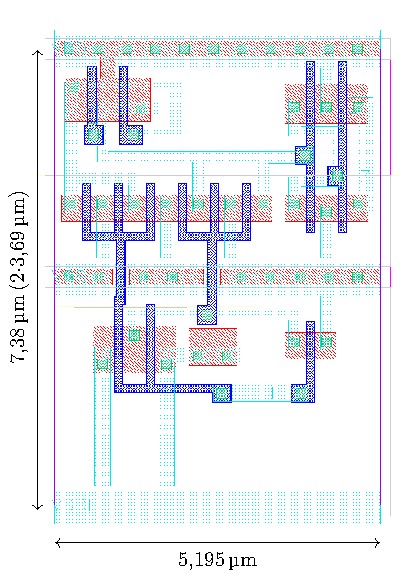
\includegraphics[scale=0.78]{slike/prezentacija/layout_lvl_lh.pdf} };
		\end{scope}
		\draw[thick, red] (2.78,-0.33) --++ (0.5,0) --++ (0,0.74) -|++ (-0.5,-0.74) ;
		\draw[->, dashed, thick, red] (3.28,0) --++ (1.4,0);
		\draw[thick, red] (4.68, -3.8) --++ (0,7.5) --++ (5.8,0) |-++ (-5.8,-7.5);
        	\end{tikzpicture}
    	\end{figure}		
\end{frame}

\subsection{Верификација \FLL-a}

\begin{frame}
	\frametitle{\secname: \subsecname\ (Двостепени режим)}
	\centering
	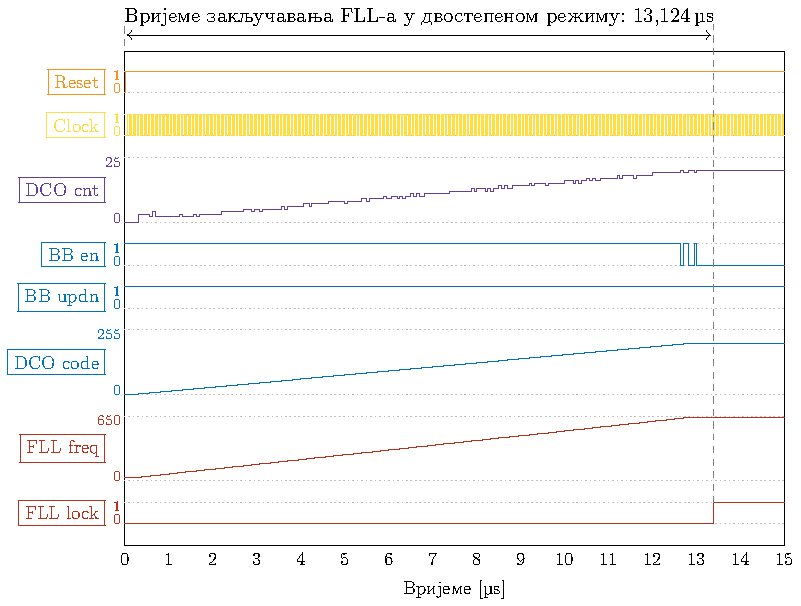
\includegraphics[scale=0.7]{slike/prezentacija/sim_BB.pdf}
\end{frame}

\begin{frame}
	\frametitle{\secname: \subsecname\ \\(\PID\ режим)}
	\begin{center}
		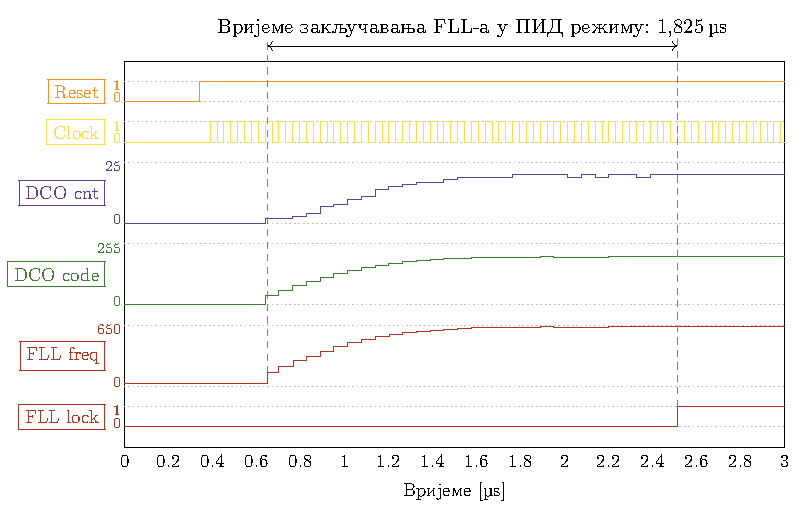
\includegraphics[scale=0.8]{slike/prezentacija/sim_PID.pdf}	
	\end{center}
\end{frame}

\subsection{PVT зависност \DCO-a}

\begin{frame}{\secname: \subsecname}
    \small
    \vspace{-0.5cm}
    \begin{itemize}
        \item Зависност (а) учестаноси осциловања и (б) корака учестаности ($K_\text{DCO}$) од броја укључених тростатичких инвертора за најспорији, типични и најбржи случај.
    \end{itemize}
    %\vspace{-1cm}
    \begin{columns}[t]
        \begin{column}{0.5\textwidth}
            \begin{figure}[!t]
            	\centering
            	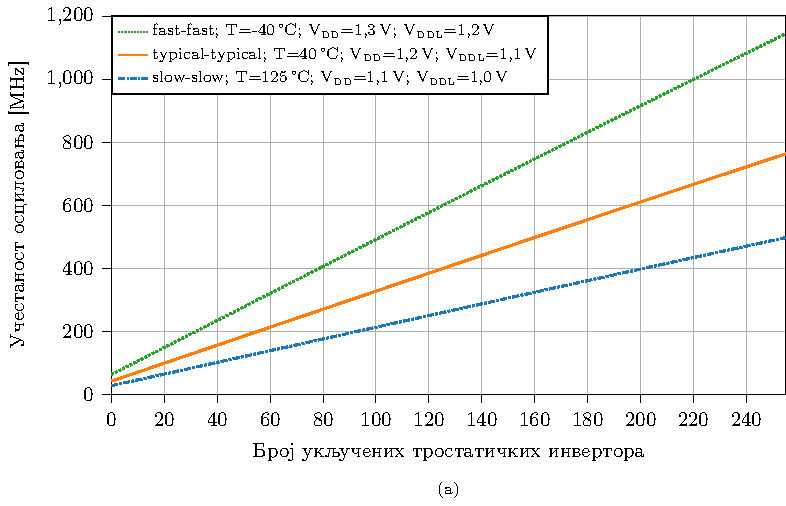
\includegraphics[scale=0.52]{slike/prezentacija/sim_DCO_worst_typical_best_freq.pdf}
            	\label{DCO_worst_typical_best_freq}
            \end{figure}
		\end{column}
		\begin{column}{0.5\textwidth}
            \vspace{0.1cm}
            \begin{figure}[!t]
                %\centering
                \includegraphics[scale=0.52]{slike/prezentacija/sim_DCO_worst_typical_best_kdco.pdf}
                \label{DCO_worst_typical_best_kdco}
            \end{figure}
		\end{column}
	\end{columns}
\end{frame}

\subsection{Временски одзив \DCO-a}

\begin{frame}{\secname: \subsecname}
    \begin{columns}[t]
        \begin{column}{0.54\textwidth}
            \begin{figure}[!t]
            	\centering
            	\includegraphics[scale=0.64]{slike/prezentacija/sim_DCO_phases.pdf}
            	\label{DCO_phases}
            \end{figure}
		\end{column}
		\begin{column}{0.46\textwidth}
	    \small
            \begin{itemize}
                \item Генерисани сигнали на 5 фаза \DCO-а у $V_\text{DD}$ и $V_\text{DDL}$ области такта.
                \item Параметри временског одзива \DCO-a \\ (за типичан \PVT\ случај):
                    \begin{itemize}
                        \item Трајање узлазне ивице: $t_\text{lh}=26\,ps$ 
                        \item Трајање силазне ивице: $t_\text{hl}=20\,ps$
                        \item Кашњење тростатичког инвертора:
                			\begin{equation}
                    			t_\text{d} = \dfrac{t_\text{lh} + t_\text{hl}}{2} = 23\,ps \nonumber
                			\end{equation}
                        \item Фазни помјерај: $t_\text{ps}=920\,ps$
                    \end{itemize}
            \end{itemize}
		\end{column}
	\end{columns}
\end{frame}

\subsection{Фазни шум \DCO-a}

\begin{frame}{\secname: \subsecname}
    \begin{itemize}
        \item Због насумичних фазних одступања, спектар снаге реалног осцилатора се шири на учестаности око учестаности носиоца $\omega_c$.
    \end{itemize}
    \begin{columns}[t]
        \begin{column}{0.5\textwidth}
            \begin{figure}[!t]
            	\centering
            	\includegraphics[scale=0.8]{slike/prezentacija/osc_noise_1_1.pdf}
            \end{figure}
		\end{column}
		\begin{column}{0.5\textwidth}
            \begin{figure}[!t]
            	\centering
            	\includegraphics[scale=0.8]{slike/prezentacija/osc_noise_1_2.pdf}
            \end{figure}
	\end{column}
    \end{columns}
\end{frame}

\begin{frame}{\secname: \subsecname}
    \begin{itemize}
        \item Извори насумичних фазних поремећаја у виду шума треперења \engl{flicker noise} и термичког шума \engl{thermal noise} манифестују се као $1/\omega^3$ and $1/\omega^2$ области, респективно.
    \end{itemize}
    \begin{figure}[!t]
	    \centering
	    \includegraphics[scale=0.7]{slike/prezentacija/osc_noise_2.pdf}
    \end{figure}
\end{frame}

\begin{frame}{\secname: \subsecname}
    \begin{itemize}
        \item Профил фазног шума \DCO-а (у типичном \PVT\ случају, за $V_\text{DDL}$=1,1\,V и $f_\text{osc}$=640\,MHz):
    \end{itemize}
    \begin{figure}[!t]
	    \centering
	    \includegraphics[scale=0.65]{slike/prezentacija/sim_DCO_phase_noise.pdf}
	    \label{DCO_phase_noise}
    \end{figure}
\end{frame}

\section{Пајтон модел \FLL-а}

\begin{frame}{\secname}
	\begin{itemize}
		\item Практичније симулирање
		\item Брже предвиђање понашања \FLL-a
		\item \underline{Параметризација понашања компоненти дизајна}
			\begin{itemize}
				\item Почетна учестаност \DCO-а
				\item Корак учестаности, $K_\text{DCO}$
			\end{itemize}
		\item Резултати симулација из Пајтон модела не морају да одговарају резултатима из симулација на нивоу логичких кола, већ су ту да пројектанта наведу на исправну употребу одређених константи (као што су \PID\ константе) или да му помогну око одабира компоненти дизајна чије појединачно понашање му је већ познато и може да се параметризује (рецимо понашање \DCO-а)
	\end{itemize}
\end{frame}

\subsection{Поређење рада управљачких режима}

%\begin{frame}{\secname: \subsecname}
%    \begin{figure}[!t]
%	    \centering
%	    \includegraphics[scale=0.75]{slike/prezentacija/py_pid_vs_cnt_2.pdf}
%    \end{figure}
%\end{frame}

\begin{frame}{\secname: \subsecname}
    \begin{figure}[!t]
	    \centering
	    \includegraphics[scale=0.75]{slike/prezentacija/py_pid_vs_cnt_1.pdf}
    \end{figure}
\end{frame}

\subsection{Утицај константи \PID\ регулатора}

\begin{frame}{\secname: \subsecname}
    \begin{figure}[!t]
	    \centering
	    \includegraphics[scale=0.8]{slike/prezentacija/py_pid_kp_tuning.pdf}
    \end{figure}
\end{frame}

\begin{frame}{\secname: \subsecname}
    \begin{figure}[!t]
	    \centering
	    \includegraphics[scale=0.8]{slike/prezentacija/py_pid_ki_tuning.pdf}
    \end{figure}
\end{frame}

\subsection{Утицај корака учестаности на одзив}

\begin{frame}{\secname: \subsecname}
    \begin{figure}[!t]
	    \centering
	    \includegraphics[scale=0.75]{slike/prezentacija/py_kdco_tuning.pdf}
    \end{figure}
\end{frame}

\section{Поређење \DCO-a у 130\texorpdfstring{\,}{ }nm и 180\texorpdfstring{\,}{ }nm TSMC технологији}

\begin{frame}{\secname}
	\begin{itemize}
		\item Скалирањем технологије транзистори постају мањи, чиме се омогућава већа густина транзистора на чипу, што даље доводи до смањења укупне површине интегрисаног кола.
		\item Ознаке 130\,nm и 180\,nm се односе на дужине полисилицијумског гејта MOSFET-а.
		\item Површине потребне за реализацију \DCO-a у 130\,nm и 180\,nm су редом 3700\,\text\textmu m$^\text2$ и 6000\,\text\textmu m$^\text2$, што значи да је умањење површине услијед скалирања око 40\,\%.
	\end{itemize}
\end{frame}

\begin{frame}{\secname}
    \begin{columns}[t]
        \begin{column}{0.4\textwidth}
            \begin{figure}[!t]
            	\centering
            	\includegraphics[scale=0.8]{slike/prezentacija/layout_dco5_hl_lh_130_2.pdf}
		\caption{Лејаут \DCO-а у 130\,nm TSMC технологији.}
            \end{figure}
		\end{column}
		\hspace{-0.8cm}
		\begin{column}{0.6\textwidth}
            \begin{figure}[!t]
            	\centering
            	\includegraphics[scale=0.8]{slike/prezentacija/layout_dco5_hl_lh_180.pdf}
		\caption{Лејаут \DCO-а у 180\,nm TSMC технологији.}
            \end{figure}
	\end{column}
    \end{columns}
\end{frame}

\begin{frame}{\secname}
\begin{table}[!ht]
	\caption{Поређење RMS вриједности потрошње струје и просјечне снаге \DCO-a пројектованих у 130\,nm и 180\,nm.}
	\centering
	\begin{tabular}{|c||c|c|}
		\hline
	        Tехнологија & 130\,nm & 180\,nm \\
		\specialrule{1.5pt}{0pt}{0pt}
		$\text{rms}(i_\text{DDL})$ & 2,185\,mA & 3,105\,mA \\
		\hline
		$\text{rms}(i_\text{DD})$ & 0,18\,mA & 0,27\,mA \\
		\hline
		Укупно rms($i$) & 2,365\,mA & 3,375\,mA \\
		\specialrule{1.5pt}{0pt}{0pt}
		$P_{avg}(V_\text{DDL})$ & 2,5\,mW & 5,0\,mW \\
		\hline
		$P_{avg}(V_\text{DD})$ & 0,22\,mW & 0,5\,mW \\
		\hline
		Укупно $P_{avg}$ & 2,72\,mW & 5,5\,mW \\
		\hline
	\end{tabular}
\end{table}
\begin{itemize}
	\item Просјечна потрошња снаге је мања за око 50\,\% у 130\,nm TSMC технологији (долази до изражаја квадратна зависност од напона напајања).
\end{itemize}
%\bigskip
%\begin{equation}
%	P = Nf_\text{OSC}C_\text{tot}V_\text{DDL}^{2} \nonumber
%\end{equation}
\end{frame}

\begin{frame}{\secname}
\begin{table}[!ht]
	\caption{Подешавање услова рада за симулације опсега учестаности.}
	%\label{tab:compare_tech:freq:cond}
	\centering
	\begin{tabular}{|c|c||c|c|c|c|}
		\hline
		Случај & Технологија & Процесни угао & Температура & $V_\text{DD}$ & $V_\text{DDL}$ \\
		\specialrule{1.5pt}{0pt}{0pt}
		Најспорији & 130\,nm & slow-slow & 125$^{\circ}\,C$ & 1,1\,V & 1,0\,V \\
		\hline
		Типични & 130\,nm & typical-typical & 40$^{\circ}\,C$ & 1,2\,V & 1,1\,V \\
		\hline
		Најбржи & 130\,nm & fast-fast & -40$^{\circ}$\,C & 1,3\,V & 1,2\,V \\
		\specialrule{1.5pt}{0pt}{0pt}
		Најспорији & 180\,nm & slow-slow & 125$^{\circ}$\,C & 1,6\,V & 1,4\,V \\
		\hline
		Типични & 180\,nm & typical-typical & 40$^{\circ}$\,C & 1,8\,V & 1,6\,V \\
		\hline
		Најбржи & 180\,nm & fast-fast & -40$^{\circ}$\,C & 2,0\,V & 1,8\,V \\
		\hline
	\end{tabular}
\end{table}
\begin{itemize}
	\item Примјећујемо значајно већи напон напајања за \DCO\ у 180\,nm.
\end{itemize}
\end{frame}

\begin{frame}{\secname}
\begin{table}[!ht]
	\caption{Поређење опсега учестаности при различитим условима рада за \DCO\ пројектован у 130\,nm и 180\,nm.}
	\centering
	\begin{tabular}{|c|c||c|c|}
		\hline
		Случај & Технологија & $f_\text{min}$ & $f_\text{max}$ \\
		\specialrule{1.5pt}{0pt}{0pt}
		Најспорији & 130\,nm & 27,2\,MHz & 502\,MHz \\
		\hline
		Типични & 130\,nm & 42\,MHz & 764\,MHz \\
		\hline
		Најбржи & 130\,nm & 63,3\,MHz & 1,146\,GHz \\
		\specialrule{1.5pt}{0pt}{0pt}
		Најспорији & 180\,nm & 23,06\,MHz & 421,4\,MHz \\
		\hline
		Типични & 180\,nm & 40\,MHz & 726\,MHz \\
		\hline
		Најбржи & 180\,nm & 64,43\,MHz & 1,168\,GHz \\
		\hline
	\end{tabular}
\end{table}
\begin{itemize}
	\item Скалирањем технологије значајно се може смањити напон напајања, а да се и даље добија жељени опсег учестаности, што значи да се уз много мању потрошњу постижу исте, или чак боље, перформансе у раду \DCO-a.
\end{itemize}
\end{frame}

\section{Утицај дубоке јаме N типа у аналогном пројектовању \DCO-а}

\begin{frame}{\secname}
	\begin{itemize}
		\item Примјењено на \DCO\ у 180\,nm технологији.
		\item NMOS транзистори нису изоловани од супртрата, па се јавља додатни шум у супстрату.
		\item У основној CMOS изради, NMOS транзистор је уроњен у P супстрат повезан на масу, док је PMOS уроњен у N јаму \engl{N-well} повезану на напајање.
	\end{itemize}
        \begin{figure}[!t]
        	\centering
            	\includegraphics[scale=0.8]{slike/prezentacija/dnw1.pdf}
		\caption{Попречни пресјек PMOS и NMOS транзистора.}
        \end{figure}
\end{frame}

\begin{frame}{\secname}
	\small
	\begin{itemize}
		\item Изолација NMOS транзистора се може постићи коришћењем поменуте дубоке јаме N типа \engl[DNW]{Deep N-Well}. Она се формира уметањем високоенергетске јонске имплантације непосредно прије формирања стандардне јаме N типа
		\item Повезивање дубоке јаме N типа врши се преко стандардне јаме N типа која је окружује и повезана је на напајање, $V_\text{DD}$. Тако се, стварањем изоловане јаме P типа \engl{P-well}, изолује NMOS транзистор.
		\item Како додатном изолацијом глобални P супстрат остаје без p$+$ споја који је неопходан да се појавом шума у супстрату не наруше перформансе уређаја, додаје се заштитни прстен који се повезује на $V_\text{SS}$.
	\end{itemize}
	\vspace{-0.3cm}
        \begin{figure}[!t]
        	\centering
            	\includegraphics[scale=0.6]{slike/prezentacija/dnw2.pdf}
        \end{figure}
\end{frame}

\begin{frame}{\secname}
	\small
	\begin{itemize}
		\item Како NMOS и PMOS транзистори обично иду у пару приликом CMOS пројектовања, да би се боље искористио простор тј. смањила површина крајњег лејаута, за повезивање дубоке јаме N типа се може искористити стандардна јама N типа коју користи PMOS транзистор, а заштитни прстен се помјера да обухвати читав дизајн.
	\end{itemize}
	\vspace{-0.3cm}
        \begin{figure}[!t]
        	\centering
            	\includegraphics[scale=0.6]{slike/prezentacija/dnw3.pdf}
        \end{figure}
	\vspace{-0.3cm}
	\begin{itemize}
		\item Како додавање дубоке јаме N типа изискује и додавање заштитног прстена, површина коју заузима дизајн се повећава, тако да то може бити недостатак овог приступа ако су захтјеви за површином строги.
	\end{itemize}
\end{frame}

\section{Резиме}
\begin{frame}{\secname}
	\begin{itemize}
	    \item Дигитални \FLL\ 
	        \begin{itemize}
		        \item Предности наспрам аналогног \FLL-a
      	        	\item Синтетизабилност из ћелија стандардне библиотеке
      	        	\item Имплементација у SystemVerilog језику за опис хардвера у 130\,nm CMOS
      	        	\item Параметризован и широко подесиви \DCO\
      	        	\item Два управљачка режима \FLL-a: ПИД и двостепени
      	        	\item Неутралисање ефеката метастабилности приликом пребацивања између различитих области такта
			\item Пајтон модел \FLL-a
			\item Поређење перформанси \DCO-а у 130\,nm и 180\,nm CMOS технологији
			\item Утицај додавања дубоке јаме N типа на потискивање шума супстрата
            	\end{itemize}
	    \bigskip
	    \item Даљи рад:
	        \begin{itemize}
	             \item Тестирање чипа након фабрикације и паковања
	             \item Имплементација додатних синтетизабилних дигиталних блокова: PLL, LDO, итд.
	        \end{itemize}        
	\end{itemize}
\end{frame}

\section{Објављени рад}

\begin{frame}{\secname}
	\vspace{-0.5cm}
        \begin{figure}[!t]
        	\centering
            	\includegraphics[scale=0.21]{slike/prezentacija/etran_1.png}
        \end{figure}
\end{frame}

\begin{frame}{\secname}
        \begin{figure}[!t]
        	\centering
            	\includegraphics[scale=0.28]{slike/prezentacija/IcETRAN2024_nagrada.pdf}
        \end{figure}
\end{frame}

\section*{Навигација за питања}
% Са "sections=..." се одређује која поглавља се приказују
{\setbeamertemplate{footline}{}\begin{frame}[noframenumbering]{\secname}
    \begin{columns}[t]
	\footnotesize
        \begin{column}{0.5\linewidth}
            \tableofcontents[sections={2-5}]
        \end{column}
        \begin{column}{0.5\linewidth}
            \tableofcontents[sections={6-}]
        \end{column}
    \end{columns}
\end{frame}}

\end{document}
